%% 
%% Copyright 2007, 2008, 2009 Elsevier Ltd
%% 
%% This file is part of the 'Elsarticle Bundle'.
%% ---------------------------------------------
%% 
%% It may be distributed under the conditions of the LaTeX Project Public
%% License, either version 1.2 of this license or (at your option) any
%% later version.  The latest version of this license is in
%%    http://www.latex-project.org/lppl.txt
%% and version 1.2 or later is part of all distributions of LaTeX
%% version 1999/12/01 or later.
%% 
%% The list of all files belonging to the 'Elsarticle Bundle' is
%% given in the file `manifest.txt'.
%% 

%% Template article for Elsevier's document class `elsarticle'
%% with numbered style bibliographic references
%% SP 2008/03/01

\documentclass[preprint,review,12pt]{elsarticle}

%% Use the option review to obtain double line spacing
%% \documentclass[authoryear,preprint,review,12pt]{elsarticle}

%% Use the options 1p,twocolumn; 3p; 3p,twocolumn; 5p; or 5p,twocolumn
%% for a journal layout:
%% \documentclass[final,1p,times]{elsarticle}
%% \documentclass[final,1p,times,twocolumn]{elsarticle}
%% \documentclass[final,3p,times]{elsarticle}
%% \documentclass[final,3p,times,twocolumn]{elsarticle}
%% \documentclass[final,5p,times]{elsarticle}
%% \documentclass[final,5p,times,twocolumn]{elsarticle}

%% For including figures, graphicx.sty has been loaded in
%% elsarticle.cls. If you prefer to use the old commands
%% please give \usepackage{epsfig}

%% The amssymb package provides various useful mathematical symbols
\usepackage{amssymb}
\usepackage[caption=false,font=footnotesize]{subfig}
\usepackage{multirow}
\usepackage{capt-of}
\usepackage{algpseudocode}


  
 % \usepackage{cite}
%% The amsthm package provides extended theorem environments
%% \usepackage{amsthm}

%% The lineno packages adds line numbers. Start line numbering with
%% \begin{linenumbers}, end it with \end{linenumbers}. Or switch it on
%% for the whole article with \linenumbers.
%% \usepackage{lineno}

\journal{TO ADD}

\begin{document}

\begin{frontmatter}

%% Title, authors and addresses

%% use the tnoteref command within \title for footnotes;
%% use the tnotetext command for theassociated footnote;
%% use the fnref command within \author or \address for footnotes;
%% use the fntext command for theassociated footnote;
%% use the corref command within \author for corresponding author footnotes;
%% use the cortext command for theassociated footnote;
%% use the ead command for the email address,
%% and the form \ead[url] for the home page:
%% \title{Title\tnoteref{label1}}
%% \tnotetext[label1]{}
%% \author{Name\corref{cor1}\fnref{label2}}
%% \ead{email address}
%% \ead[url]{home page}
%% \fntext[label2]{}
%% \cortext[cor1]{}
%% \address{Address\fnref{label3}}
%% \fntext[label3]{}

\title{PaMPa-HD: EXTENSION - TO MODIFY}

%% use optional labels to link authors explicitly to addresses:
%% \author[label1,label2]{}
%% \address[label1]{}
%% \address[label2]{}

\author[label1]{Daniele Apiletti,
Elena Baralis,
Tania Cerquitelli, \\
Paolo Garza, Fabio Pulvirenti}
\author[label2]{and Pietro Michiardi}

\address[label1]{Dipartimento di Automatica e Informatica\\
Politecnico di Torino\\
Torino, Italy\\ Email: name.surname@polito.it}
\address[label2]{Data Science Department\\ Eurecom\\
Sophia Antipolis, France\\ Email: pietro.michiardi@eurecom.fr}
\begin{abstract}
%% Text of abstract
% %Frequent closed itemset mining is among the most complex exploratory techniques
% in data mining,
% %and provides the ability to discover hidden correlations in transactional
% datasets.
% %The explosion of Big Data is leading to new parallel and distributed
% approaches.
% %Unfortunately, most of them are designed to cope with low-dimensional datasets,
% %whereas no distributed high-dimensional frequent closed itemset mining
% algorithms exists.
% %This work introduces PaMPa-HD,
% %a parallel MapReduce-based frequent closed itemset mining algorithm
% %for high-dimensional datasets, based on Carpenter.
% %The experimental results, performed on both real and synthetic datasets,
% %show the efficiency and scalability of PaMPa-HD.
% %PaM-Car outperforms both the single-machine Carpenter implementation
% %and the best state-of-the-art distributed approaches

%Frequent closed itemset mining, a data mining technique for discovering hidden
%correlations in transactional datasets, is among the most complex exploratory
%techniques in data mining.
%Thanks to the spread of distributed and
%parallel frameworks, the development of scalable approaches able to deal with
%the so called Big Data has been extended to frequent itemset mining.
%Unfortunately, most of the current algorithms are designed to cope with
%low-dimensional datasets,
%delivering poor performances in those use cases characterized by
%high-dimensional data.
%This work introduces PaMPa-HD, a parallel MapReduce-based frequent closed
%itemset mining algorithm for high dimensional datasets.
%The experimental results, performed on two real-life high-dimensional use cases,
%show the efficiency of the proposed approach in terms of execution time, load balancing and robustness to memory issues.




In today's world, large volumes of data are being continuously
generated by many scientific applications, such as bioinformatics or networking.
Since each monitored event is usually characterized by a variety of features,
high-dimensional datasets have been continuously generated. 
To extract value from these complex collections of data, different exploratory data mining algorithms
can be used to discover hidden and non-trivial correlations among data.
Frequent closed itemset mining is an effective but computational expensive 
technique that is usually used to support data exploration. 
Thanks to the spread of distributed and
parallel frameworks, the development of scalable approaches able to deal with
the so called Big Data has been extended to frequent itemset mining.
Unfortunately, most of the current algorithms are designed to cope with
low-dimensional datasets,
delivering poor performances in those use cases characterized by
high-dimensional data.
This work introduces PaMPa-HD, a MapReduce-based frequent closed
itemset mining algorithm for high dimensional datasets.
An efficient solution has been proposed to 
parallelize and speed up the mining process. Furthermore, different strategies have been proposed to easily configure the algorithm parameter.
The experimental results, performed on real-life high-dimensional use cases,
show the efficiency of the proposed approach in terms of execution time, load balancing and robustness to memory issues.

\end{abstract}

\begin{keyword}
%% keywords here, in the form: keyword \sep keyword

%% PACS codes here, in the form: \PACS code \sep code

%% MSC codes here, in the form: \MSC code \sep code
%% or \MSC[2008] code \sep code (2000 is the default)

\end{keyword}

\end{frontmatter}

%% \linenumbers

%% main text
\section{Introduction}
\label{Introduction}
In the last years, the increasing capabilities of recent applications
to produce and store huge amounts of information,
the so called "Big Data"~\cite{Jin201559}, have changed dramatically
the importance of the intelligent analysis of data.
Data mining, together with machine learning~\cite{DBLP:journals/bdr/Al-JarrahYMKT15}, 
is considered
one of the fondamental tools on which Big Data analytics
are based.
In both academic and industrial domains, the interest towards data mining,
which focuses on extracting effective and usable knowledge from large
collections of data, has risen.
The need for efficient and highly scalable data mining tools increases with the
size of the datasets,
as well as their value for businesses and researchers aiming at extracting
meaningful insights increases.\\
Frequent (closed) itemset mining is among the most complex exploratory
techniques in data mining.
It is used to discover frequently co-occurring items
according to a user-provided frequency threshold, called minimum support.
Existing mining algorithms revealed to be very efficient on simple datasets
but very resource intensive in Big Data contexts.
In general, the application of data mining techniques to Big Data collections
is characterized by the need of huge amount of resources.
For this reason, we are witnessing the explosion of parallel and distributed
approaches,
typically based on distributed frameworks, such as Apache Hadoop~\cite{HDFS}
and Spark~\cite{Zaharia_spark}.
As clearly shown in Chapter \ref{survey}, unfortunately, most of the scalable distributed techniques
for frequent itemset mining have been designed to cope with datasets
characterized by few items per transaction (low dimensionality, short
transactions). Their design, on the contrary, focuses on very large datasets in terms of number of
transactions.
Currently, only single-machine implementations exist to address very long
transactions,
such as Carpenter~\cite{Zaki_Carpenter}, and no distributed implementations at
all.\\
%Nevertheless, many researchers in scientific domains such as bioinformatics or
%networking,
%often require to deal with this type of data.
Nevertheless, many scientific applications, such as bioinformatics or networking, 
generate a large number of events characterized by a variety of features.
Thus, high-dimensional datasets have been continuosly generated.
For instance, most gene expression datasets are characterized by
a huge number of items (related to tens of thousands of genes)
and a few records (one transaction per patient or tissue).
Many applications in computer vision deal with high-dimensional data, such as
face recognition.
An increasing portion of big data is actually related to geospatial data~\cite{Lee201574} and
smart-cities. Some studies have built this type of large datasets
measuring the occupancy of different car lanes:
each transaction describes the occupancy rate in a captor location and in a
given timestamp~\cite{PEMSDataset}.
In the networking domain, instead,
the heterogeneous environment provides many different datasets
characterized by high-dimensional data,
such as URL reputation, advertising, and social network
datasets~\cite{snapnets}.
To effectively deal with those high-dimensional datasets,
novel and distributed approaches are needed.

This work introduces PaMPa-HD \cite{pampa_v1}, \cite{pampa_pulvi},
a parallel MapReduce-based frequent closed itemset mining algorithm
for high-dimensional datasets.
PaMPa-HD relies on the Carpenter algorithm~\cite{Zaki_Carpenter}. 
The PaMPa-HD design\footnote{The source code of PaMPa-HD can be downloaded from https://github.com/fabiopulvi/PaMPa-HD},through an ad-hoc synchronization technique, takes into account crucial design aspects,
such as load balancing and robustness to memory-issues. Furthermore, different strategies have been proposed to easily tune up the parameter configuration.
The algorithm has been thoroughly evaluated on real high dimensional datasets. 
PaMPa-HD outperforms the state-of-the-art distributed approaches
in execution time and by supporting lower minimum support threshold. 


The paper is organized as follows:
Section~\ref{Preliminaries} briefly reintroducess the frequent (closed) itemset mining
problem,
Section~\ref{Carpenter algorithm} briefly describes the centralized version
of Carpenter,
and Section~\ref{Distributed implementation outline} presents the proposed
PaMPa-HD algorithm.
Section~\ref{Experiments} describes the experimental evaluations
proving the effectiveness of the proposed technique,
Section~\ref{Applications} discusses possible applications of PaMPa-HD and, finally, Section~\ref{Conclusion} introduces future works and conclusions.
%Section~\ref{Related work} presents a brief review of the state of the art,
%and Section~\ref{Applications} discusses possible applications of PaMPa-HD.
%Finally, Section~\ref{Conclusion} introduces future works and conclusions.





\section{Frequent itemset mining background}
\label{Preliminaries}

\begin{figure}[!t]
%\renewcommand{\arraystretch}{1.3}
%\centerline
{\subfloat[Horizontal representation of $\mathcal{D}$]{
\label{horizontalexampledataset}
\begin{tabular}{|c|l|}
\hline
\multicolumn{2}{|c|}{$\mathcal{D}$}\\
\hline
\hline
	tid & items \\
\hline
	1 & a,b,c,l,o,s,v \\
\hline
	2 & a,d,e,h,l,p,r,v \\
\hline
	3 & a,c,e,h,o,q,t,v \\
\hline
	4 & a,f,v \\
\hline
	5 & a,b,d,f,g,l,q,s,t \\
\hline
\end{tabular}}}%
\hfil
{\subfloat[Transposed representation of $\mathcal{D}$]{
\label{TTexampledataset}
\begin{tabular}{|l|l|}
\hline
\multicolumn{2}{|c|}{$TT$}\\
\hline
\hline
	item & tidlist \\ \hline
	a & 1,2,3,4,5 \\ \hline
	b & 1,5 \\ \hline
	c & 1,3 \\ \hline
	d & 2,5 \\ \hline
	e & 2,3 \\ \hline
	f & 4,5 \\ \hline
	g & 5 \\ \hline
	h & 2,3 \\ \hline
	l & 1,2,5 \\ \hline
	o & 1,3 \\ \hline
	p & 2 \\ \hline
	q & 3,5 \\ \hline
	r & 2 \\ \hline
	s & 1,5 \\ \hline
	t & 3,5 \\ \hline
	v & 1,2,3,4 \\ \hline
\end{tabular}}}%
\hfil
{\subfloat[$TT|_{\{2,3\}}$: example of con\-di\-tio\-nal
tran\-spo\-sed table]{
\label{conditionalexampledataset}
\begin{tabular}{|l|l|}
\hline
\multicolumn{2}{|c|}{$TT|_{\{2,3\}}$}\\
\hline
\hline
item & tidlist \\ \hline
a &4,5 \\ \hline
e & - \\ \hline
h & -\\ \hline
v &4 \\ \hline
\end{tabular}}}%
\caption{Running example dataset $\mathcal{D}$}
\label{exampledataset}
\end{figure}
%
%Let $\mathcal{I}$ be a set of items. A transactional dataset $\mathcal{D}$
%consists of a set of transactions $\{t_1, \dots, t_n\}$,
%where each transaction $t_i\in \mathcal{D}$ is a set of items (i.e.,
%$t_i\subseteq \mathcal{I}$)
%and it is identified by a transaction identifier ($tid_i$).
%Figure~\ref{horizontalexampledataset} reports an example of a transactional
%dataset with 5 transactions.
%It is used as a
%running example through the paper.
%
%An itemset $I$ is defined as a set of items (i.e., $I\subseteq\mathcal{I}$) and
%it is characterized by a tidlist and a support value.
%The tidlist of an itemset $I$, denoted by $tidlist(I)$, is defined as the set of
%tids of the transactions in $\mathcal{D}$ containing $I$,
%while the support of $I$ in $\mathcal{D}$, denoted by $sup(I)$, is defined as
%the ratio between the number of transactions in $\mathcal{D}$ containing $I$
%and the total number of transactions in $\mathcal{D}$ (i.e.,
%$|tidlist(I)|/|\mathcal{D}|$).
%For instance, the support of the itemset \textit{\{aco\}} in
%the running example dataset $\mathcal{D}$ is 2/5 and its tidlist is $\{1,3\}$.
%An itemset $I$ is considered frequent if its support is greater than a
%user-provided minimum support threshold $minsup$.
%
%Given a transactional dataset $\mathcal{D}$ and a minimum support threshold
%$minsup$, the Frequent Itemset Mining \cite{KumarBook} problem consists in
%extracting the complete set of frequent itemsets from $\mathcal{D}$.
%In this paper, we focus on a valuable subset of frequent itemsets called
%frequent closed itemsets~\cite{Zaki_Carpenter}. Closed itemsets
%allow representing the same information of traditional frequent itemsets in a
%more compact form.
%In addition, an item or itemset $I$ is closed in  $\mathcal{D}$ if there exists no superset that
%has the same support count as  $I$.\\
%For instance, in our running example, given a $minsup=2$, the itemset \textit{\{ab\}} is a frequent itemset (support=2), but it is not closed for the presence of the itemset \textit{\{abls\}} (support=2). 
%% %If an itemset is frequent, all of its subsets are frequent for the
%% \textit{monotonic property}.
%% %For the same rule, if an items or an itemset is not frequent, none of its
%% supersets are frequent. In addition, an items
%% % or itemset $I$ is closed in  $\mathcal{D}$ if there exists no superset that
%% has the same support count as  $I$.\\
Since Frequent Itemset Mining preliminaries were introduced far before in the dissertation,
let us just recall and deepen the key concepts fundamental to better understand PaMPa-HD and its
enumeration tree-based exploration strategy.

As already mentioned, a transactional dataset can also be represented in a vertical format, which is
usually a more effective representation of the dataset when the average number
of items per transactions is orders of magnitudes larger than the number of
transactions.
This representation, called \textit{transposed table} $TT$, assumes that each
row consists of an item $i$ and its list of transactions, i.e.,
$tidlist(\{i\})$. Let $r$ be an arbitrary row of $TT$, $r.tidlist$ denotes the
tidlist of row $r$.
Figure~\ref{TTexampledataset} reports the transposed representation of the
running example reported in Figure~\ref{horizontalexampledataset}.

Given a transposed table $TT$ and a tidlist $X$, the conditional transposed
table of $TT$ on the tidlist $X$, denoted
by $TT|_{X}$, is defined as a transposed table such that:
(1) for each row $r_i\in TT$ such that $X\subseteq r_i.tidlist$ there exists one
tuple $r_i^{\prime}\in TT|_{X}$ and
(2) $r_i^{\prime}$ contains all tids in $r_i.tidlist$ whose tid is higher than
any tid in $X$.
For instance, consider the transposed table $TT$ reported in
Figure~\ref{TTexampledataset}. The
projection of $TT$ on the tidlist \textit{\{2,3\}} is the transposed table
reported in Figure~\ref{conditionalexampledataset}.
Each transposed table $TT|_{X}$ is associated with an itemset composed by the
items in $TT|_{X}$.
For instance, the itemset associated with $TT|_{\{2,3\}}$ is \textit{\{aehv\}}
(see Figure~\ref{conditionalexampledataset}).


% %Given a row or a set of rows (in the sequel, \textit{row set}) $x$, $TT|_{x}$,
% is the projection of the whole vertical datasets on the row set x. Each
% transposed table is associated with an itemset composed of the items in the
% table. For each item, the associated tidlist is composed of the tids greater
% than any tid in the row set x. For instance, $TT|_{2,3}$ in tab 3 is the
% transposed table of the row set \textit{2,3} and it represents the itemset
% \textit{aehv}.




%%% Inizio sezione algoritmo
% \section{Algorithms}
% \label{Distributed Carpenter}
% This Section presents the centralized version of
% Carpenter~\cite{Zaki_Carpenter}
% and the proposed PaM-Car algorithm.

\section{The Carpenter algorithm}
\label{Carpenter algorithm}
%As discussed in section \ref{Related work}, t
The most popular techniques to perform itemset mining (e.g.,
Apriori~\cite{Agr94} and FP-growth~\cite{Han00}) adopt the itemset enumeration
approach (see Section \ref{survey_centralized} for further discussion).
% to mine the frequent itemsets.
However, itemset enumeration revealed to be ineffective with datasets with a
high average number of items per transactions \cite{Zaki_Carpenter}.
%Apriori algorithm, in fact, has a very high number of candidates to generate
%and to count, while the trees generated by FP-Growth-based approaches hardly
%fit in main memory.
%In conclusion, these algorithms were not developed for the use cases related
% to high number of features, focusing on high number of transactions.\\
To tackle this problem, the Carpenter algorithm~\cite{Zaki_Carpenter} was
proposed.
Specifically, Carpenter is a frequent itemset extraction algorithm devised to
handle datasets characterized by a relatively small number of
transactions but a huge number of items per transaction.
To efficiently solve the itemset mining problem, Carpenter adopts an effective
depth-first transaction enumeration approach based on the transposed
representation of the input dataset.
To illustrate the centralized version of Carpenter, we will use the running
example dataset $\mathcal{D}$ reported in Figure~\ref{horizontalexampledataset},
and
more specifically, its transposed version (see Figure~\ref{TTexampledataset}).
%Before going deeper into the algorithm explanation, some preliminary
% information will be provided to facilitate the reader comprehension.
%Let us start saying that the algorithm assumes to process a vertical
%transposition of the input dataset.
%Carpenter assumes to process a transposed representation of the input dataset.
Recall that in the transposed
representation each row of the table consists of an item $i$ with its tidlist.
For instance,
the last row of Figure~\ref{TTexampledataset} shows that item \textit{v}
appears in
transactions 1, 2, 3, 4.
%The rows are sorted in a numerical order (oppure The tids in each tidlist are
%sorted in a numerical orders?).
%From the initial transposed table TT, given x as a row or a row set,
%  $x$, $TT|_{x}$, is the projection of the whole vertical datasets on the
%row or the row set $x$, as defined in section \ref{Preliminaries}.\\


\begin{figure}[!t]
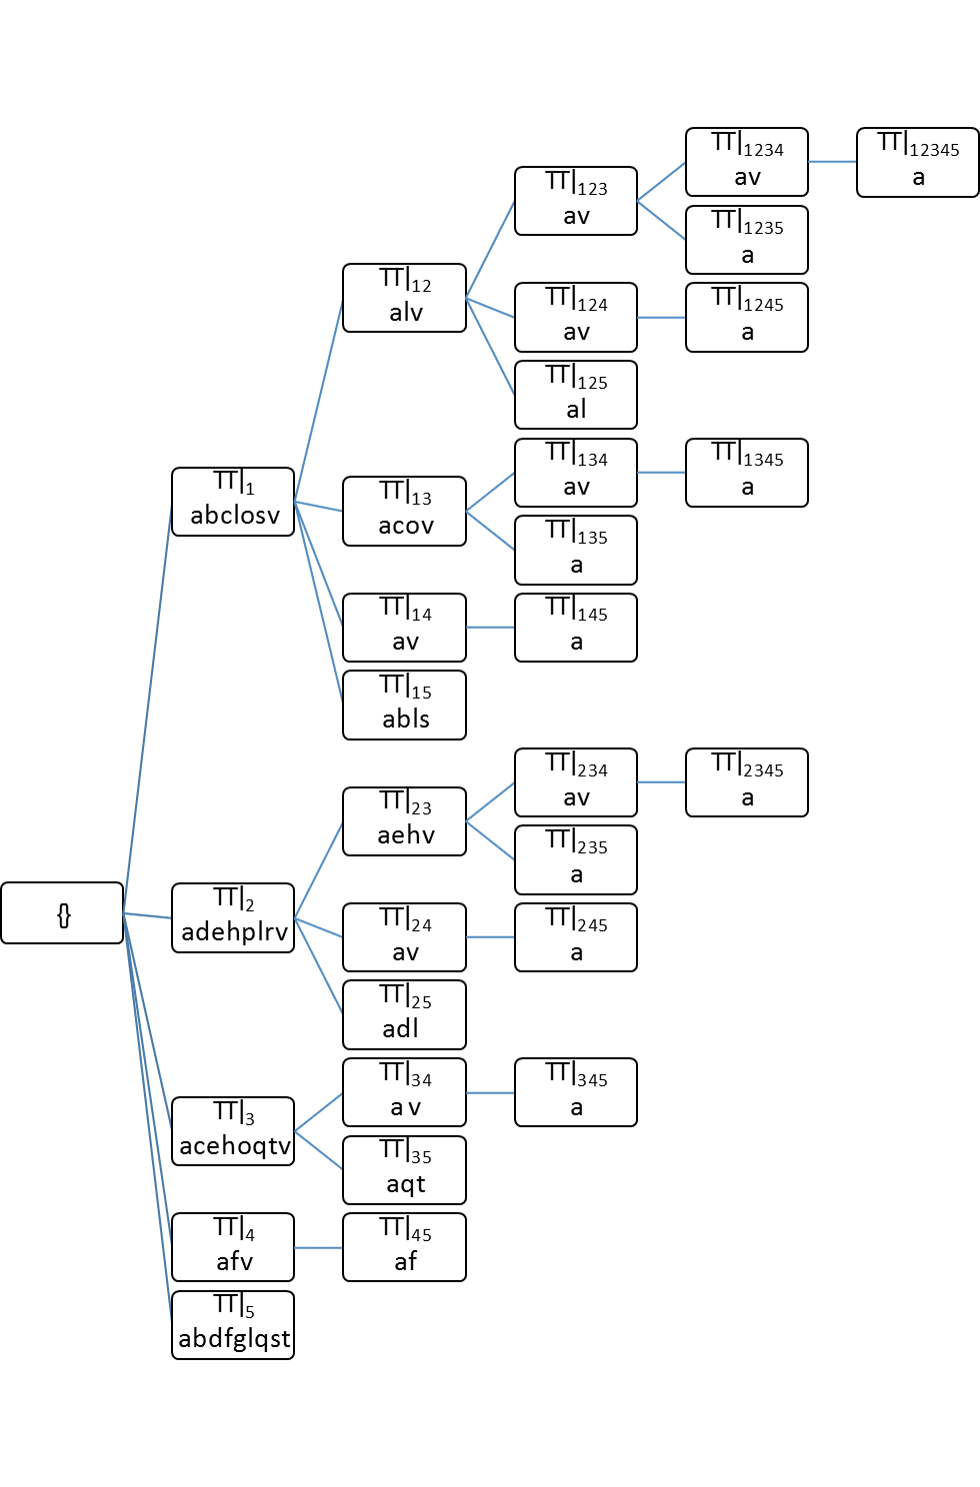
\includegraphics[width=4in]{chapters/pampa/running_example1.png}
\caption{The transaction enumeration tree of the running example dataset in
Figure~\ref{horizontalexampledataset}. For the sake of clarity, no pruning rules
are applied to the tree.}
\label{running_1}
\end{figure}

%Conditional transposed tables and the depth first enumeration of the
%transactions are the core of Carpenter. Specifically,
Basically, Carpenter builds a transaction enumeration tree by exploiting a set of pruning rules
which avoid the expansion of useless branch of the tree. 
In the tree, each node corresponds to a
conditional transposed table $TT|_X$ and its related information (i.e., the
tidlist $X$ with respect to which the conditional transposed table is built and
its associated itemset).
The transaction enumeration tree, when pruning techniques are not applied,
contains all the tid combinations (i.e., all the possible
tidlists $X$).
Figure~\ref{running_1} reports the
transaction enumeration tree obtained by processing the running example dataset.
To avoid the generation of duplicate
tidlists, the transaction enumeration tree is built by exploring the tids in
lexicographical order (e.g., $TT|_{\{1,2\}}$ is generated instead of
$TT|_{\{2,1\}}$).
Each node of the tree is associated with a conditional transposed table on a
tidlist.
For instance, the conditional transposed table
$TT|_{\{2,3\}}$ in Figure~\ref{conditionalexampledataset}, matches the node
$\{2,3\}$ in Figure~\ref{running_1}.


%The enumeration tree is built from initial transposed table: in figure
%\ref{running_1}, a full exploration of the tree based on initial transposed
%table is shown. Each node of the tree, as already said, matches a transposed
%table over a row set. In our example, the transposed table$TT|_{2,3}$ in
%figure 3, matches the node 2,3 in figure \ref{running_1}.
Carpenter performs a depth first search (DFS) of the enumeration tree to mine the set
of frequent closed itemsets.
%Visiting the tree in this way, adopting a pruning branch policy that will
%be detailed in the following, leads to the extraction of the complete
%frequent closed itemset set without duplicates (details and proofs can be
%found in \cite{Zaki_Carpenter}).
%We will describe the Carpenter algorithm by means of the running example.
Referring to the tree in Figure~\ref{running_1}, the depth first search would
lead to the visit of the nodes in the following order:
\{1\}, \{1,2\}, \{1,2,3\}, \{1,2,3,4\}, \{1,2,3,4,5\}, \{1,2,3,5\}, \{...\}.
For each node, Carpenter applies a procedure that decides if the itemset
associated with that node is a frequent closed itemset or not.
%Specifically, for each node, Carpenter decides if the itemset associated with
%the current node is a frequent closed  itemset
%by considering: 1) the tidlist $X$ associated with the node, 2) the conditional
%transposed table
%$TT|_{X}$, 3) the set of frequent closed itemsets found up to the current step
%of the tree search, and 4) the enforced minimum support threshold ($minsup$).
%The first information is useful to enforce the DFS exploration and to check the 
%actual support of the itemset; the conditional transposed table is used to obtain
% the itemset associated to the node, while the remaing tids are useful to determine
% how and if the node should be expanded. The frequent closed itemsets found (3)
% are used to avoid to process the same itemset twice; due to the enumeration tree 
%architecture, the real support of the itemset is the one obtained the first time the 
%itemset is processed in a DFS exploration manner. Finally, the enforced minsup 
%support threshold is used to decide if the itemset is a frequent closed itemset.
Specifically, for each node, Carpenter decides if the itemset associated with
the current node is a frequent closed  itemset
by considering: \begin{enumerate}
\item The tidlist $X$ associated with the node, useful to enforce the depth-first exploration and to check the actual support of the itemset
\item The conditional transposed table $TT|_{X}$, used to obtain the itemset associated to the node and, through the remaing tids, determine how and if the node should be expanded
\item The set of itemsets found up to the current step of the tree search, used to avoid to process the same itemset twice (due to the enumeration tree architecture, the real support of the itemset is the one obtained the first time the itemset is processed in a depth-first exploration manner)
\item The enforced minimum support threshold ($minsup$), used to decide if the itemset is a frequent closed itemset
\end{enumerate}
Based on the theorems reported in~\cite{Zaki_Carpenter}, if the itemset $I$
associated with the current node is a frequent closed itemset then $I$
is included in the frequent closed itemset set. Moreover, by exploiting the
analysis performed on the current node, part of the remaining search space
(i.e.,
part of the enumeration tree) can be pruned, to avoid the analysis of nodes that
will never generate new closed itemsets.
To this purpose, three pruning rules are applied on the enumeration tree, based
on the evaluation performed on the current node and the associated
transposed table $TT|_{X}$:
\begin{itemize}
\item \textbf{Pruning rule 1.} If the size of $X$, plus the number of distinct
tids in the rows of $TT|_{X}$ does not reach the minimum support threshold,
the subtree rooted in the current node is pruned.
\item \textbf{Pruning rule 2.} If there is any tid $tid_i$ that is present in
all the tidlists of the rows of $TT|_{X}$, $tid_i$ is deleted from $TT|_{X}$.
The number of discarded tids is updated to compute the correct support of the
itemset associated with the pruned version of $TT|_{X}$.
\item \textbf{Pruning rule 3.} If the itemset associated with the current node
has been already encountered during the depth first search,
the subtree rooted in the current node is pruned because it can never generate
new closed itemsets.
\end{itemize}

%Rule 3 is the most effective pruning rule, especially considering the
%distributed implementation detailed in \ref{Distributed implementation
%outline}. It allows to prune the branches related to already found itemsets,
%that represents a waste of computation time and memory.
%After the pruning phase, the support of the itemset is compared with the
%minsup. The support is identified by the number of row ids composing $X$,
%plus the number of rows discarded by the second pruning rule. If the support
%is greater or equal than the minsup, as shown in figure 5, the itemset
%is added to the set of frequent closed ones.

The tree search continues in a depth first fashion moving on the next node of
the enumeration tree. More specifically,
let $tid_l$ be the lowest tid in the tidlists of the current $TT|_{X}$, the next
node to explore is the one associated with
$X^\prime=X\cup \{tid_l\}$.


Among the three rules mentioned above, pruning rule 3 assumes a global knowledge
of the enumeration tree explored in a depth first manner.
This, as detailed in section~\ref{Distributed implementation outline}, is very
challenging in a distributed environment that adopts a shared-nothing
architecture, like the one we address in this work.



% %versione 2
% %\\
% %Carpenter algorithm is based on the depth first exploration of a row
% enumeration tree. A running example of the enumeration tree built on the dataset
% in table 1 is represented in figure \ref{running_1}. A transposed table
% $TT|_{x}$ is the projection of the whole vertical datasets on the row set x, as
% defined in \ref{Preliminaries}. Each transposed table is associated with an
% itemset composed of the items in the table. For each item, the associated
% tidlist is composed of the tids greater than any tid in the row set x. Each
% table represents a node in the row enumeration tree. For instance, $TT|_{2,3}$
% in tab 3 corresponds to the node 2 3 in the enumeration tree.
% %\\The tree exploration corresponds to a recursive processing of the transposed
% tables, generating adding a tid to the row set in depth first manner. Exploring
% the tree in this way, applying a set of pruning rules detailed in a few lines,
% leads to the extraction of all the closed itemsets (details and proofs can be
% found in \cite{Zaki_Carpenter}). The first iteration processes the whole
% vertical dataset. Each iteration, given a transposed table $TT|_{x}$ as input,
% can be resumed in:
% %\begin{enumerate}
% %\item apply pruning rules
% %\item if the support is over the minsup, add the related itemset to the set of
% frequent closed itemsets
% %\item expand the table adding a tid in the row set, following a depth first
% manner
% %\item start a new recursion with the new table
% %\end{enumerate}
% %The pruning rules allow to prune some branches without exploring all the
% possible tid combinations. The most effective is the rule used to prune some
% branches of the tree if the related itemsets have already been found in the tree
% exploration. The rules are:
% %\begin{itemize}
% %\item \textbf{Pruning rule 1:} If the row of the projection, plus the potential
% rows in the tid lists do not reach the minimum support threshold, the table is
% discarded and the branch is pruned.
% %\item \textbf{Pruning rule 2:} If there is any row id which is present in all
% the tid lists, it is deleted from the table. The number of discarded rows is
% updated.
% %\item \textbf{Pruning rule 3:} If the itemset characterizing the table has been
% already seen in the tree, the branch is pruned.
% %\end{itemize}
% %The process continues recursively until there is no table to expand and all the
% closed itemsets have been found. A most detailed explanation and theoretical
% proofs are in \cite{Zaki_Carpenter}.

\begin{figure}[!t]
%\centering
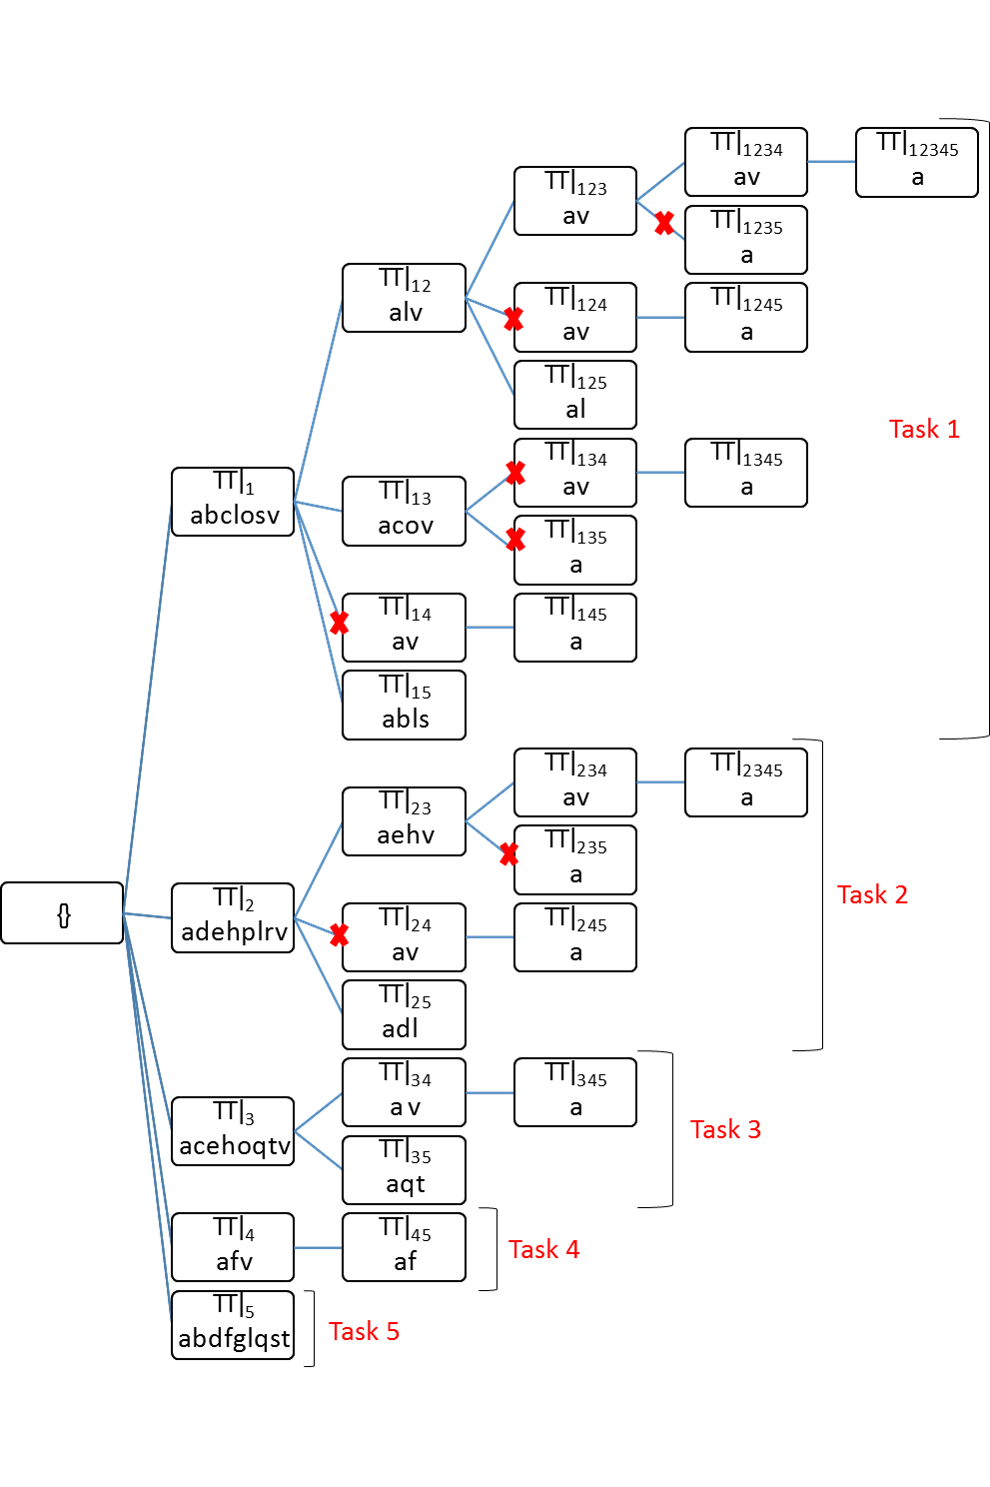
\includegraphics[width=4in]{chapters/pampa/running_example2_d.png}
% where an .eps filename suffix will be assumed under latex,
% and a .pdf suffix will be assumed for pdflatex; or what has been declared
% via \DeclareGraphicsExtensions.
\caption{Running toy example: each node expands a branch of the tree
independently. For the sake of clarity, pruning rule 1 and 2 are not applied. The pruning rule 3 is
applied only within the same task: the small crosses on the edges represent pruned
nodes due to local pruning rule 3, e.g.
the one on node \{2 4\} represents the pruning of node \{2 4\}.}
\label{running_2}
\end{figure}




\section{The PaMPa-HD algorithm}
\label{Distributed implementation outline}
In this section we describe the new algorithm, called PaMPa-HD, proposed in this paper. Specifically, 
we describe how PaMPa-HD parallelizes the itemset mining
process and applies the pruning rules discussed in Section~\ref{Carpenter algorithm} in a parallel 
environment.
Furthermore, we discuss how, through an ad-hoc
synchronization phase, PaMPa-HD achieves a good load balancing
and robustness to memory issues.

As discussed in the previous section, given the complete enumeration tree (see Figure~\ref{running_1}), the
centralized Carpenter algorithm
extracts the whole set of closed itemsets by performing a depth first search
(DFS) of the tree.
%By tracing the set of closed itemsets encountered by traversing the tree,
%Carpenter also prunes part of the search space by applying the three pruning
%rules illustrated above. 
%described in Section~\ref{Carpenter algorithm}.
Differently, in order to parallelize the mining process, the PaMPa-HD algorithm splits the depth
first search process in a set of (partially) independent
sub-processes, that autonomously evaluate sub-trees of the search space.
%PaMPa-HD exploits the pruning rules 1 and 2 and a slight variation of the 
%pruning rule 3 discussed in Section~\ref{Carpenter algorithm}.
Specifically, the whole problem can be split by assigning
each subtree rooted in $TT|_{X}$, where $X$ is a single transaction id in the
initial dataset, to an independent sub-process.
Each sub-process applies the centralized version of Carpenter on its conditional
transposed table $TT|_{X}$ and extracts a subset of the final closed itemsets.
The subsets of closed itemsets mined by each sub-process
are merged to compute the whole closed itemset result.
Since the sub-processes are independent, they can be executed in parallel by
means of a distributed computing platform, e.g., Hadoop.
Figure~\ref{running_2} shows the application of the proposed approach on the
running example.
Specifically, five independent sub-processes are executed in the case of the
running example, one for each row (transaction) of the original dataset.
The crosses on the nodes represent the local pruning within each parallel task.
Partitioning the enumeration tree in sub-trees allows processing bigger
enumeration trees with respect to the centralized version. However, this
approach does not allow fully exploiting pruning rule 3
because each sub-process works independently and is not aware of the partial
results (i.e., closed itemsets) already extracted by the other sub-processes.
Hence, each sub-process can only prune part of its own search space by
exploiting its ``local'' closed itemset list, while
it cannot exploit the closed itemsets already mined by the other sub-processes.
For instance, Task T2 in Figure~\ref{running_2} extracts the closed itemset $av$
associated with node $TT|_{2, 3, 4}$.
However, the same closed itemset is also mined by T1 while evaluating node
$TT|_{1, 2, 3}$.
In the centralized version of Carpenter, the duplicate version of $av$
associated with node $TT|_{1, 2, 4}$ is not generated because $TT|_{1, 2, 4}$
follows
$TT|_{1, 2, 3}$ in the depth first search, i.e., the tasks are serialized and
not parallel.

Since pruning rule 3 has a high impact on the reduction of the search space, its
inapplicability leads to a negative
impact on the execution time of the distributed algorithm (see Section~\ref{Experiments} for further details).
To address this issue, we share partial results among the sub-processes.
Each independent sub-process analyzes only a part of the search subspace.
Then, when a maximum number of visited nodes is reached, the partial results are
synchronized through a synchronization phase. Of course, the exploration of the
tree finishes also when the subspace has been completely explored.
%Each sub-process analyzes only a part the search subspace, then, when memory is
%full or when a maximum number of visited nodes is reached, it stores on disk
%(e.g., in HDFS, the Hadoop distributed file system) the partial set of closed
%itemset mined so far and the remaining sub-tree left to analyze.

Specifically, the sync phase filters the partial results (i.e., nodes of the tree
still to be analyzed and found closed itemsets) globally applying pruning rule
3. The pruning strategy consists of two phases.
In the first one, all the transposed tables and the already found closed
itemsets are analyzed. The transposed tables and the closed itemsets related to
the same itemset are grouped together in a bucket. For instance, in our running
example, each element of the bucket $B_{av}$ can be:
\begin{itemize}
\item a frequent closed itemset $av$ extracted during the subtree exploration of
the node $TT_{3, 4}$,
\item a transposed table associated to the itemset $av$ among the ones that
still have to be expanded (nodes  $TT_{1, 2, 3}$ and  $TT_{2, 3, 4}$).
\end{itemize}
We remind the readers that, because of the independent nature of the Carpenter
subprocesses, the elements related to the same itemset can be numerous, because
obtained in different subprocesses. Please note that all the extracted closed
itemsets come together with the tidlist of the node in which they have been
extracted.

In the second phase, in order to respect the depth-first pruning strategy of the
rule 3, for each bucket it is kept only the oldest element (transposed table or
closed itemset) based on a depth-first order. The depth-first sorting of the
elements can be easily obtained comparing the tidlists of the elements of the
bucket.
Therefore, in our running example from the
bucket $B_{av}$, it is kept the node $TT_{1, 2, 3}$ (See Figure~\ref{running_3b}) .
The transposed tables which are not pruned in this phase are then expanded to continue the enumeration tree exploration.


Afterwards, a new set of sub-processes is defined from the filtered results,
starting a new iteration of the algorithm. In the new iteration, the Carpenter
tasks process also the frequent closed itemsets obtained in the previous iteration,
which are used to enrich the local memory of the task and enhance the effectiveness of the local pruning. 
The Carpenter tasks
process the remaining transposed tables, that are expanded, as before, until the
maximum number of processed tables is reached. In order to enhance the
effectiveness of the pruning rules related to the local Carpenter task, the
tables are processed in a depth-first order. After that, as before, in the
synchronization phase, pruning rule 3 is applied.
%A synchronization and pruning task works on the partial results
%of the sub-processes to globally apply pruning rule 3
%on the remaining search subspaces, i.e.,
%on the remaining nodes of the enumeration tree.
%After the application of the synchronization and pruning step,
%a new set of sub-processes is defined,
%for each remaining node of the enumeration tree.
%that is a descendant of one of the nodes analyzed during the first iteration a
%new process is instantiated and executed.
The overall process is applied iteratively by instantiating new sub-processes
and synchronizing their results,
until there are no nodes left.
The application of this approach to our running example is represented in
Figure~\ref{running_3}, in which the small crosses represent the pruning related to the local
state memory; and in Figure~\ref{running_3b}, in which the bigger crosses represent the pruning related to the synchronization phase.
The table related to the itemset \textit{av}
associated with the tidlist/node \{2, 3, 4\} is pruned because the
synchronization
job discovers a previous table with the same itemset,
i.e.  the node associated with the transaction ids combination \{1, 2, 3\}.
The use of this approach allows the parallel execution of the mining process,
providing at the same time a very high reliability dealing with heavy
enumeration trees, which can be split and pruned according to pruning rule 3.
Of course, this architecture cannot deliver the same pruning efficiency characterizing the centralized implementation of Carpenter in which the complete tree depth-first exploration is known.

The introduction of the sync phase leads also to a better load balancing of the tasks. At each synchronization, the tables to process are redistributed among the tasks. Therefore, the task related to the first branches of the tree, which are the ones with more nodes than others, are splitted into several subtasks. In this way, as shown Section~\ref{Experiments}, we achieve a better exploitation of the resources.


\begin{figure}[!t]
%\centering
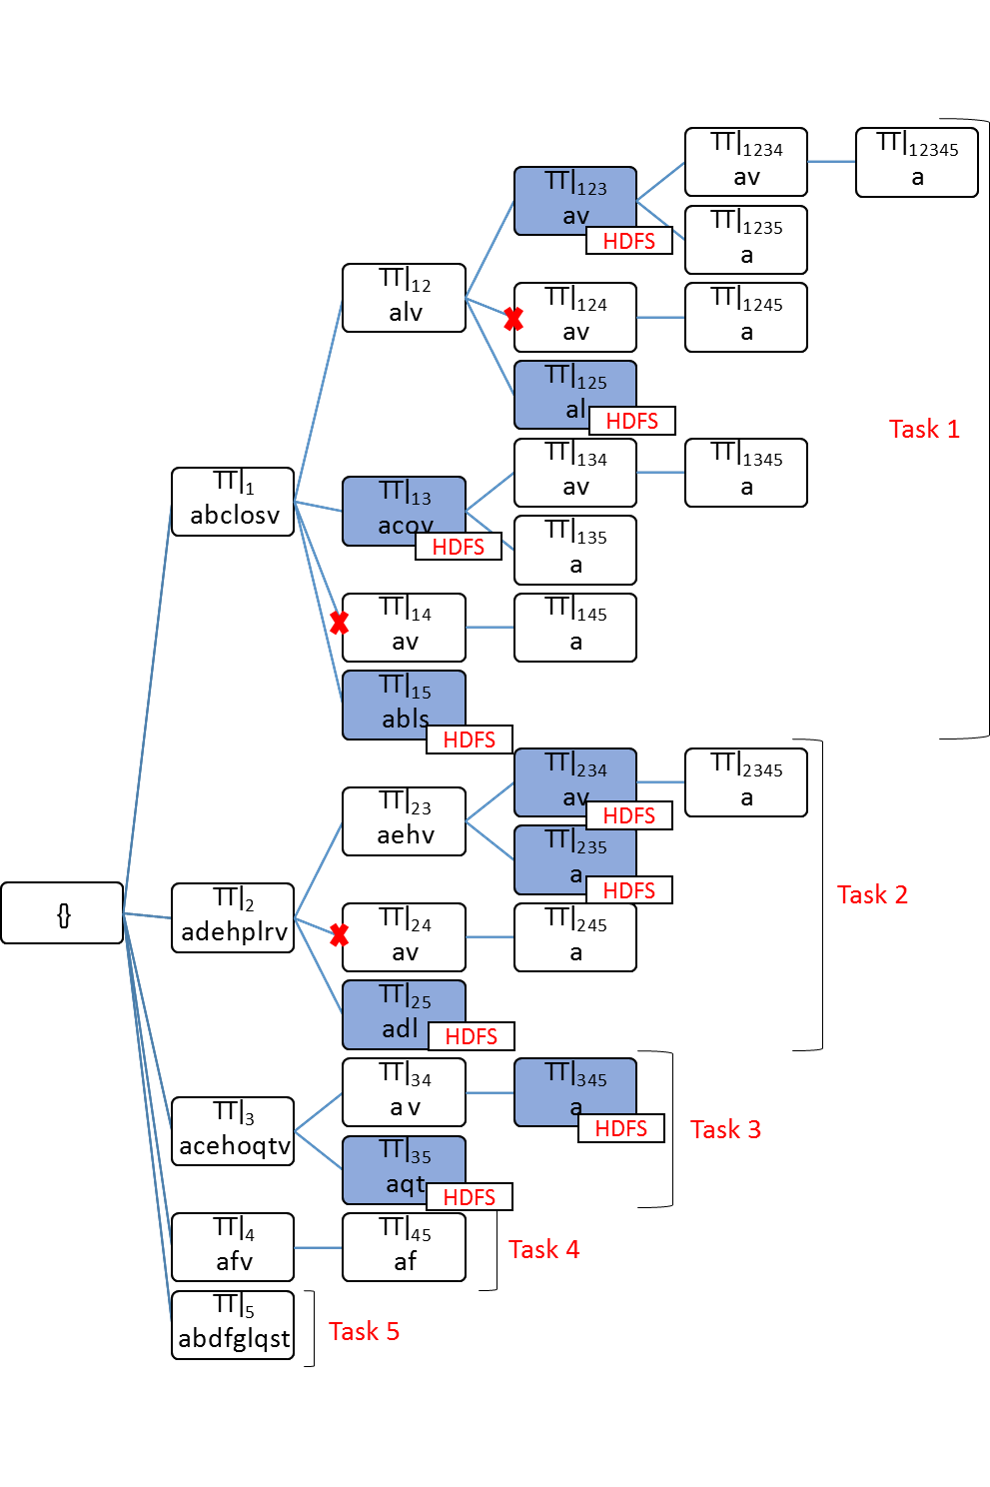
\includegraphics[width=4in]{chapters/pampa/running_example3_d_A.png}
% where an .eps filename suffix will be assumed under latex,
% and a .pdf suffix will be assumed for pdflatex; or what has been declared
% via \DeclareGraphicsExtensions.
\caption{Execution of PaMPa-HD on the running example dataset.
For the sake of clarity, pruning rules 1 and 2 are not
applied. The dark nodes represent the nodes that have been written to HDFS in
order to apply the synchronization job.}

%The red crosses on nodes represent that the nodes have been removed by the
%local pruning, e.g.,
%the one on node \{2 4\} represents the pruning of node \{2 4\}.

\label{running_3}
\end{figure}

\begin{figure}[!t]
%\centering
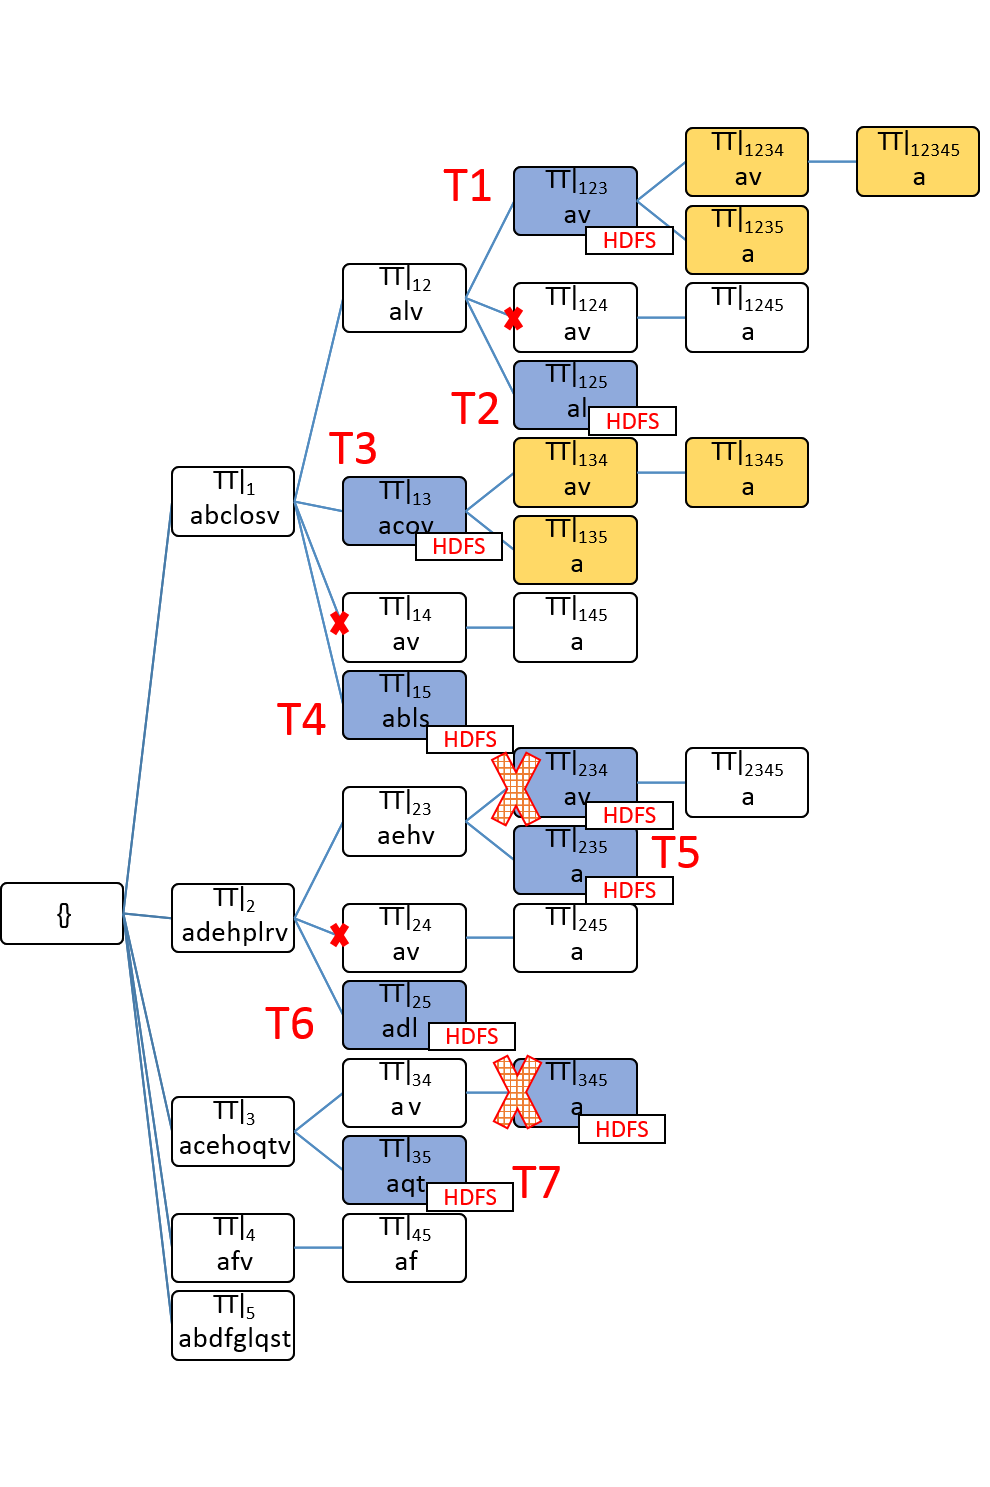
\includegraphics[width=4in]{chapters/pampa/running_example3_d_B_quadretti.png}
% where an .eps filename suffix will be assumed under latex,
% and a .pdf suffix will be assumed for pdflatex; or what has been declared
% via \DeclareGraphicsExtensions.
\caption{Execution of PaMPa-HD on the running example dataset.
For the sake of clarity, pruning rules 1 and 2 are not
applied. The big checked crosses on nodes represent the nodes which have been
removed by the synchronization job, e.g.,
the one on node \{2 3 4\} represents the pruning of node \{2 3 4\}.}
\label{running_3b}
\end{figure}

%Each worker node does not
%run Carpenter to the end but stops and writes intermediate results to the disk.
%After that, the redundancy is deleted with a synchronization job and Carpenter
%starts again from the filtered tables, handled in parallel by different tasks.




%
%\fbox{\parbox{0.9\linewidth}{
%PaMPa-HD pseudo code
% \begin{algorithmic}[1]
%
% \Procedure{PaMPa-HD}{$minsup;$ $initial$ $TT$}
%
%
%\State Job 1 Mapper: process each row of TT \par
%and send it to reducers, using as key values \par the tids of the tidlists
%
%\State Job 1 Reducer: aggregates $TT|_{x}$ and run \par local Carpenter until
%expansion threshold is \par reached  or memory is not enough
%\State Job 2 Mapper: process all the closed itemset \par or transposed
% tables from the previous job \par and send them to reducers
%\State Job 2 Reducer: for each itemset belonging \par to a table or a frequent
%closed, keep \par the eldest in  a Depth First fashion
%\State Job 3 Mapper: process each closed itemset \par and $TT|_{x}$ from  the  previous job. \par For the transposed tables run
%local Carpenter \par until  expansion  threshold is reached
%\State Job 3 Reducer: for each itemset belonging \par to a table or a frequent
%closed, keep \par the eldest in  a Depth First fashion
%\State Repeat Job 3 until no more \par conditional tables  need to be
%processed
%% \Procedure{PaMPa-HD}{$minsup;$ $initial$ $TT$}
%%
%%
%%\State Job 1 Mapper: process each row of TT \par
%%and send it to reducers, using as key values \par the tids of the tidlists
%%
%%\State Job 1 Reducer: aggregates $TT|_{x}$ and run \par local Carpenter until
%%expansion threshold is \par reached  or memory is not enough
%%\State Job 2 Mapper: process all the closed itemset \par or transposed
%% tables from the previous job \par and send them to reducers
%%\State Job 2 Reducers: for each itemset belonging \par to a table or a frequent
%%closed, keep \par the eldest in  a Depth First fashion
%%\State Job 3 Mapper: process each $TT|_{x}$ from  the \par previous job and run
%%Local Carpenter until \par expansion  threshold is reached  or memory \par is not
%%enough
%%\State Repeat Job 2 and Job 3 until no more \par conditional tables  need to be
%%processed
%
%
%
%
% \EndProcedure
% \end{algorithmic}
%
%}}
%% \caption{PaMPa-HD pseudo code}
% \label{alg1}

\subsection{Implementation details}
\label{MapReduce Carpenter}
PaMPa-HD implementation uses the Hadoop MapReduce framework.
The algorithm consists of three MapReduce jobs as shown in PaMPa-HD pseudocode
(Algorithm~\ref{alg1}).

\begin{algorithm}[t]
\scriptsize
\centering
\caption{PaMPa-HD at a glance}
 \label{alg1}
%\fbox{\parbox{0.9\linewidth}{
 \begin{algorithmic}[1]
 \Procedure{PaMPa-HD}{$minsup;$ $initial$ $TT$}
\State Job 1 Mapper: process each row of TT \par
and send it to reducers, using as key values \par the tids of the tidlists

\State Job 1 Reducer: aggregate $TT|_{x}$ and run \par local Carpenter until
expansion threshold is \par reached  or memory is not enough
\State Job 2 Mapper: process all the closed itemset \par or transposed
 tables from the previous job \par and send them to reducers
\State Job 2 Reducer: for each itemset belonging \par to a table or a frequent
closed, keep \par the eldest in  a Depth First fashion
\State Job 3 Mapper: process each closed itemset \par and $TT|_{x}$ from  the
previous job. \par For the transposed tables run
local Carpenter \par until  expansion  threshold is reached
\State Job 3 Reducer: for each itemset belonging \par to a table or a frequent
closed, keep \par the eldest in  a Depth First fashion
\State Repeat Job 3 until there are no more \par conditional tables

 \EndProcedure
 \end{algorithmic}
%}
%}
\end{algorithm}

% \caption{PaMPa-HD pseudo code}


The Job 1, whose pseudocode is reported in Algorithm~\ref{job1},
 is developed to distribute the input dataset to the independent
tasks,
which will run a local and partial version of the Carpenter algorithm. 
The second job performs the synchronization of the partial results and 
exploits the pruning rules. At the end, the last job interleaves the Carpenter
execution with the synchronization phase.\\


\textbf{Job 1} (Algorithm~\ref{job1}). Each mapper is fed
with a transaction of the input dataset, which is supposed to be in a vertical
representation, together with the minsup parameter. As detailed in
Algorithm~\ref{job1}, each transaction is in the form $item,tidlist$.
For each transaction, the mapper performs
the following steps. For each tid $t_{i}$ of the input tidlist, given
$TL_{greater}$ the set of tids $(t_{i+1},t_{i+2},...,t_{n})$ greater than the
considered tid $t_{i}$ (lines 2-7 in Algorithm~\ref{job1}).
\begin{itemize}
%\item If $|TL_{greater}|+1 <= minsup$, output a key-value pair
%\textless key= $t_{i}$; value= $TL_{greater}$, item\textgreater,
%then analyze $t_{i+1}$ of the tidlist.
\item If $|TL_{greater}| >= minsup$, output a key-value pair \textless key=
$t_{i}$; value= $TL_{greater}$, item\textgreater, then analyze $t_{i+1}$ of the
tidlist.

 \item Else discard the tidlist.
\end {itemize}
 For instance, if the input transaction is the tidlist of item b (b, 1 2 3) and
 minsup is 1, the mapper will output three pairs:  \textless key=1; value=2 3,
 b\textgreater,  \textless  key=2; value=3, b\textgreater,  \textless  key=3;
 value=b\textgreater .\\
 After the map phase, the MapReduce shuffle and sort phase aggregates the
 \textless key,value\textgreater pairs and delivers to reducers the nodes of the
 first level of the tree, which represent the transposed tables projected on a
 single tid (lines 10-13 in Algorithm~\ref{job1}). The tables in Figure~\ref{examplejob1} illustrate the processing of
a row of the initial Transposed  representation of $D$.
Given that each key matches a single transposed table $TT_{X}$, each
reducer builds the transposed tables with the tidlists contained in the
``value'' fields.


From this table, a local Carpenter routine is run (line 14 in Algorithm~\ref{job1}). Carpenter recursively processes a transposed
table expanding it in a depth-first manner (see Section~\ref{Carpenter algorithm} for further details). 
However, the local Carpenter routine stops when the number of processed transposed tables is over the given maximum
expansion threshold. This allows periodically performing the synchronization among the parallel tasks and
hence enforcing pruning rule~3.
All the intermediate results of the local invocation of the Carpenter routine are written to HDFS (lines 15-17 in Algorithm~\ref{job1}).
%\textbf{Fabio: Ho un po' uniformato questo recap ma nn so se eliminarlo}
%The Reducer routine of Job 1, can be resumed in these phases:
% \begin{enumerate}
% \item The transposed table is composed using the tidlists from each key-value
% and a local Carpenter job is run (lines 10-14 in Algorithm~\ref{job1})
% \item For each table a local Carpenter is run. At each recursion of the Carpenter main routine, a counter is incremented: \begin{enumerate}
%\item if the counter is below the threshold, another Carpenter recursion is
%scheduled (lines 14 in Algorithm~\ref{job1})
%\item else, Carpenter main routine is not invoked anymore but all the
% intermediate results are written to HDFS (lines 15-17 in Algorithm~\ref{job1})
%\end{enumerate}
%\end{enumerate}

During the local Carpenter process, the found closed itemsets and the explored
branches are
 stored in memory in order to apply a local pruning. The closed itemsets are
emitted as output at the end of the task, together with the tidlist of the node
of the tree in
which they have been found (lines 18-20 in Algorithm~\ref{job1}). This information is required by the synchronization
phase in order to establish which element is the eldest in a depth first
exploration, i.e., which element is visited  first in a depth first
exploration (e.g. the node associated with tidlist \{1, 2,
3, 5\} is eldest than the node associated with tidlist \{2, 3, 4\} in a depth-first exploration order).\\

\begin{algorithm}[H]
\scriptsize
\centering

\caption{Dataset distribution and local and partial Carpenter execution (Job 1)}
 \label{job1}
 \begin{algorithmic}[1]
  \Procedure{Mapper}{$minsup; item_{i};tidlist$ $TL$}
\For{$j =  0$  to $|(TL)|-1$}
 \par tidlist $TL_{greater}$ : set of tids greater than \par the considered tid
$t_{j}$.
% %\State $Output(  \textless itemset;tidlist$ $+$ $table$ $content$  \Statex
% \pushcode[0] $/support) \textgreater) $
% \If{ $|TL_{greater}|+1 \ge minsup$}
\If{ $|TL_{greater}| \ge minsup$}
 \State output \textless key= $t_{j}$; value= $TL_{greater}$, item\textgreater
 \Else $ $ Break
 \EndIf
\EndFor
\EndProcedure
%\Procedure{Reducer}{$key= tid$ $X, value=list$ $of$ $tidlists$ $TL[$ $]$}
\Procedure{Reducer}{$key= tid$ $X, value=tidlists$ $TL[$ $]$}
\State Create new transposed table $ TT|_{X} $
\For{\textbf{each} tidlist $TL_{i}$ of $TL[$ $]$}
%\State  add $TL_{i}$ to $ TT|_{row_{i}} $ (populate the transposed table)
\State  add $TL_{i}$ to $ TT|_{X} $ (populate the transposed table)
\EndFor

\State Run $Carpenter (minsup;  TT|_{X}; max\_exp)$ 

%\State\hspace{\algorithmicindent}Output (Frequent Closed itemsets)
%\State\hspace{\algorithmicindent} Output (Transposed tables)
%\State\hspace{\algorithmicindent}$Output( \textless frequent$
%$closed$ $itemsets\textgreater )$
%\State\hspace{\algorithmicindent}$Output \textless itemset;$ $tidlist+Transposed
%Table$ $I$ $rows  \textgreater$
\For{\textbf{each} transposed table I found but not processed}
\State $Output \textless itemset;$ $tidlist+Transposed
Table$ $I$ $rows  \textgreater$
\EndFor
\For{\textbf{each} frequent closed itemset found}
\State $Output(  \textless itemset;tidlist+support \textgreater) $
\EndFor
 \EndProcedure
 \end{algorithmic}
\end{algorithm}

\begin{figure}[]
%\renewcommand{\arraystretch}{1.3}
%\centerline
{\subfloat[Transposed representation of $\mathcal{D}$: tidlist of item $a$]{
\label{TTexampledataset_}
\begin{tabular}{|l|l|}
\hline

	item & tidlist \\ \hline
	a & 1,2,3,4,5 \\ \hline
\end{tabular}}}%
\hfil
{\subfloat[Emitted key-value entries from the example row in Table
\ref{TTexampledataset} ]{
\label{key-value}
\begin{tabular}{|l|l|}
\hline

%\multicolumn{2}{|c|}{$TT|_{\{2,3\}}$}\\
%\hline
%\hline
key & value\\ \hline
1 & 2,3,4,5 \textbar  a \\
 \hline
2 & 3,4,5 \textbar  a \\ \hline
3 & 4,5 \textbar  a\\ \hline
4 &5 \textbar  a \\ \hline
5 & - \textbar  a \\ \hline
\end{tabular}}}%
\hfil
{\subfloat[key-value entries for key $3$]{
\label{key-value 3}
\begin{tabular}{|l|l|}
\hline
%\multicolumn{2}{|c|}{$TT|_{\{2,3\}}$}\\
%\hline
%\hline
key & value\\ \hline
3 & 4,5 \textbar a \\ \hline
3 & - \textbar c \\ \hline
3 & - \textbar e \\ \hline
3 & - \textbar h \\ \hline
3 & - \textbar o \\ \hline
3 & 5 \textbar  q \\ \hline
3 & 5 \textbar  t \\ \hline
3 & 4 \textbar  v \\ \hline
\end{tabular}}}%
\hfil
{\subfloat[$TT|_{\{3\}}$: composed with the received values]{
\label{composed_tt}
\begin{tabular}{|l|l|}
\hline
\multicolumn{2}{|c|}{$TT|_{\{3\}}$}\\
\hline
\hline
item & tidlist \\ \hline
a &4,5 \\ \hline
c & - \\ \hline
e & -\\ \hline
h & -\\ \hline
o & -\\ \hline
q & 5\\ \hline
t & 5\\ \hline
%t & 5\\ \hline
v &4 \\ \hline
\end{tabular}}}%
\caption{Job 1 applied to the running example dataset ($minsup=1$): local Carpenter algorithm
is run from the Transposed Table \ref{composed_tt}. }
\label{examplejob1}
\end{figure}



\textbf{Job 2} (Algorithm~\ref{job2}). The synchronization phase is a straightforward
MapReduce job in which mappers input is the output of the previous job: it is
 composed of the closed frequent itemsets found in the previous Carpenter tasks
 and intermediate transposed tables that still have to be expanded. The itemsets
 are associated to their minsup and the tidlist related to the node of the tree
 in which they have been found; the transposed tables are associated to the
table content,
 the corresponding itemset and the table tidlist. 
\begin{itemize}
\item For each table, the mappers output a pair of the form
\textless key=itemset; value=tidlist,table\_rows\textgreater  (lines 2 - 5 of Algorithm~\ref{job2}); 
\item for each itemset, the mappers output a pair in the form \textless
key=itemset; value=tidlist,minsup\textgreater (lines 6 - 11 of Algorithm~\ref{job2}).
\end{itemize}
 The shuffle and sort phase
 delivers to the reducers the pairs aggregated by keys. The reducers, which
match the buckets introduced in Section~\ref{Distributed implementation
outline}, compare the
 entries and emit, for the same key or itemset, only the oldest version in a
 depth first exploration (lines 15 - 21 of Algorithm~\ref{job2}). For instance, referring to our running example in
Figure~\ref{running_3b}, in the reducer related to the itemset $av$ are collected the
entries related to the nodes $T_{1 2 3}$ and $T_{2 3 4}$. Since the tidlist $1 2
3$ is previous than $2 3 4$ in a depth-first exploration order, the reducer
keeps and emits only the entry related to the node $T_{1 2 3}$.
 With this design, the redundant tables that can be obtained due to the independent nature of the Carpenter tasks, which can explore nodes related to the same itemsets, are discarded. This pruning is very
similar to the one
 performed in centralized memory at the cost of a very MapReduce-like job (similar to a \textit{WordCount} application).\\


\textbf{Job 3} (Algorithm~\ref{job3}). This is a mixture of the two previous
jobs. In the Map phase all the remaining tables
are expandend by a local Carpenter routine. The Reduce phase, instead, applies
the same kind of synchronization that is run in the synchronization job. The job
has two types of input: transposed tables and frequent closed itemsets. The
former are processed respecting a depth-first sorting and expanded until it is
reached the maximum expansion threshold (line 5 of Algorithm~\ref{job3}). From that moment, the tables are not
expanded but sent to the reducers (lines 6 - 8 of Algorithm~\ref{job3}). Please note that the tree exploration
processing the initial transposed tables in a depth-first order is the same
to a centralized architecture, enhancing the impact of pruning rule 3 (which strongly relies on this exploration manner).
The latter (i.e. the frequent closed itemsets of the previous PaMPa-HD job) are
processed in the following way. If in memory there is already an oldest
depth-first entry of the same itemset, the closed itemset is discarded. If there
is not, it is saved into memory  and used to improve the local pruning
effectiveness (lines 2 - 3). At the end of the task, all the frequent closed itemsets found are sent to
the reducers, where the redundant elements are pruned.
This job is iterated until all the transposed tables have been processed.





Thanks to the introduction of a global synchronization phase (Job 2 and
Job 3 in Algorithms 3 and 4),
the proposed PaMPa-HD approach is able to apply pruning rule 3
and handle high-dimensional datasets,
otherwise not manageable due to memory issues.



\begin{algorithm}[H]
\centering
\scriptsize
\caption{Synchronization Phase and exploitation of the pruning rule 3 (Job 2)}
  \label{job2}
 \begin{algorithmic}[1]
  \Procedure{Mapper}{$Frequent$ $Closed$ $itemset;$\par $Transposed$ $table$}
\If {Input $I$ is a table}
\State $itemset\gets ExtractItemset(I)$
\State $tidlist\gets ExtractTidlist(I)$
\State $Output(  \textless itemset;$ $tidlist+table$ $I$ $rows  \textgreater) $
\Else $ $  (i.e. input $I$ is a frequent closed Itemset)
\State $itemset\gets ExtractItemset(I)$
\State $tidlist\gets ExtractTidlist(I)$
\State $support\gets ExtractSupport(I)$
\State $Output(  \textless itemset;tidlist+support \textgreater) $
\EndIf

\EndProcedure
\Procedure{Reducer}{$key=itemset;$\par$value=itemsets$ $\&$ $tables$ $T[$ $]$}
\State $oldest\gets null$
\For{\textbf{each} itemset or table $T$ of  $T[$ $]$}
\State $tidlist\gets ExtractTidlist(T)$
%\If { $tidlist$ previous of $oldest$ in a DFS}
\If { $tidlist$ previous of $oldest$ in a Depth-First Search}
 \State $oldest\gets T$
\EndIf
\EndFor
\State $Output(\textless itemset+oldest\textgreater )$
%% \pushcode[0] $/support) \textgreater) $
% %
 \EndProcedure
 \end{algorithmic}
\end{algorithm}

\begin{algorithm}[H]
\scriptsize
\centering
\caption{Interleaving of the Carpenter execution and synchronization phase (Job 3)}
 \label{job3}
 \begin{algorithmic}[1]
  \Procedure{Mapper}{$Frequent$ $Closed$ $itemset; Transposed$ $table$}
\If {Input $I$ is a frequent closed itemset}
\State save $I$ to local memory

\Else $ $ (i.e. input $I$ is a Transposed Table)
%\State $itemset\gets ExtractItemset(I)$

\State Run $Carpenter (minsup;  TT|_{X};max\_exp)$

\For{\textbf{each} transposed table I found but not processed}
\State $Output \textless itemset;$ $tidlist+Transposed
Table$ $I$ $rows  \textgreater$
\EndFor


%\State\hspace{\algorithmicindent} $Output(  \textless itemset;tidlist+support \textgreater) $
\EndIf
\For{\textbf{each} frequent closed itemset found}
\State $Output(  \textless itemset;tidlist+support \textgreater) $
\EndFor
\EndProcedure
\Procedure{Reducer}{$key=itemset;$\par$value=itemsets$ $\&$ $tables$ $T[$ $]$}
\State $oldest\gets null$
\For{\textbf{each} itemset or table $T$ of  $T[$ $]$}
\State $tidlist\gets ExtractTidlist(T)$
%\If { $tidlist$ previous of $oldest$ in a DFS}
\If { $tidlist$ previous of $oldest$ in a Depth-First Search}
 \State $oldest\gets T$
\EndIf
\EndFor
\State $Output(\textless itemset+oldest\textgreater )$
%% \pushcode[0] $/support) \textgreater) $
% %
 \EndProcedure
 \end{algorithmic}
\end{algorithm}


%%%%%%%%%%%%% Fine sezione algoritmo
%
%\section{Expansion Threshold tuning}
%\label{threshold}
%Before the comparison with the state of the art distributed algorithms in Section~\ref{Experiments}, we performed a set of experiments to measure the performance impact of the maximum expansion threshold, evaluating the quality of a set of proposed strategies. This set of experiments, together with the ones in Section~\ref{Experiments}, are performed on two real life datasets.
The first real dataset is the \textbf{Kent Ridge Breast Cancer}~\cite{breast_cancer_dataset}, which contains gene expression data.
It is characterized by 97 rows that represent patient samples, and
24,482 attributes related to genes. The attributes are numeric (integers, floating point).
Data have been discretized with an equal depth partitioning
using 20 buckets (similarly to \cite{Zaki_Carpenter}).
The second real dataset is the \textbf{PEMS-SF} dataset~\cite{breast_cancer_dataset}, 
which describes the occupancy rate of different car lanes of San Francisco bay area freeways.
Each transaction represents the daily traffic rate of 963 lanes, sampled every 10 minutes.
It is characterized of 440 rows (in some experiments we have utilized only the first 100) and 138672 attributes (6 x 24 x 963), and it has been discretized in
equi-width bins of 0.002.
Because of their distribution and their discretizazion process, the Breast Cancer dataset is more sparse (low correlation among the dataset transactions) than the PEMS-SF dataset. 
The other two datasets were synthetically generated and tuned to simulate
use cases characterized by extremely high-dimensional data,
i.e., with massive numbers of features.
Both datasets consists of 30 transactions.
Dataset~\#1 has 1,000,000 different items
and an average transaction length of 500,000 items,
while
Dataset~\#2 is 10 times larger, with 10,000,000 different items
and an average transaction length of 5,000,000 items
(see Table~\ref{datasets}).
The discretized version of the real dataset and the synthetic dataset generator
are publicly available at http://dbdmg.polito.it/PaMPa-HD/. \textbf{TO DO: aggiungere versione finale discretized pemsf}



\begin{table}[h!]
\begin{center}
\caption{Datasets}
\label{datasets}
\begin{tabular}{|c|c|c|c|}
\hline
	Dataset & Number of  & Number of & Average number  \\
	 & transactions &different items & of items  \\ 
	  &  & &  per trasanaction  \\ \hline
	Kent Ridge Breast    & 97 & 489,640    & 24,492 \\
     CancerDataset      &    &            &  \\ \hline
PEMS-SF    & 440& 5,454,414     & 138,672 \\
     Dataset      & (100 rows version)   &   (3,946,646)       &  \\ \hline
	Synthetic Dataset \#1 & 30 & 1,000,000  & 500,000\\ \hline
	Synthetic Dataset \#2 & 30 & 10,000,000 & 5,000,000\\ \hline
\end{tabular}
\end{center}
\end{table}


PaMPa-HD is implemented in Java 1.7.0\_60 using the Hadoop MR API.
Experiments were performed on a cluster of 5 nodes running Cloudera
Distribution of Apache Hadoop (CDH5.3.1).
Each cluster node is a 2.67 GHz six-core Intel(R) Xeon(R) X5650 machine
with 32 Gbyte of main memory
running Ubuntu 12.04 server with the 3.5.0-23-generic kernel.


\subsection{Impact of the maximum expansion threshold}\label{exp_fisso}
As already mentioned in Section~\ref{Distributed implementation outline}, the maximum expansion threshold
($max\_exp$) parameter indicates the maximum number of nodes 
to be explored before a preemptive stop of each distributed sub-process is forced.
This parameter strongly affects the enumeration tree exploration,
forcing each parallel task to stop before completing the visit of its sub-tree 
and write partial results on HDFS. 
This approach allows the synchronization job to globally apply 
pruning rule 3 and reduce the search space.
Low values of $max\_exp$ threshold decrease the risks of memory issue, 
because the global problem is split into simpler and less memory-demanding
sub-problems, and facilitate the application of pruning rule 3, 
hence a smaller subspace is searched.
However, higher values allow a more efficient execution,
by limiting the start and stop of distributed tasks
(similarly to the context switch penalty), and the synchronization overheads.

In order to assess the impact of the expansion threshold parameter, we performed two set of experiments. In the first one we have performed the mining on the PEMS-SF (100 transactions) dataset with a Minsup 50, by varying $max\_exp$ from 10 to 100,000,000.  The minsup value was empirically selected in order to let the mining problem being deep enough to show up different performances. 
In Figure~\ref{pems_fixed} are shown the results in terms of execution time and number of iterations 
(i.e., the number of jobs).

It is clear how the $max\_exp$ parameter can influence the performance, with wall-clock times that can be doubled with different configurations. The best performance in terms of execution time is achieved with a maximum
expansion threshold equal to 10,000 nodes. With lower values, the execution times are slightly longer, while there is an evident performance degradation with higher $max\_exp$ values. 
This result highlights the importance of the synchronization phase.
Increasing the $max\_exp$ parameter makes the number of iterations decreasing,
but more useless tree branches are explored,
because pruning rule 3 is globally applied less frequently.
Lower values of  $max\_exp$, instead, raising the number of iterations
, introduce a slight performance
degradation caused by iterations overheads.
%With very high values of  $max\_exp$, the running time and the number of
%iterations are stable because the bottleneck becomes the free available
%memory, and the synchronization job is
%automatically applied, independently of the value of  $max\_exp$.

\begin{figure}[!t]
\includegraphics[width=5in]{immagini_extension/pems_fixed.png}
\caption{Execution time and number of iterations for different $max\_exp$ values on PEMS-SF dataset with $minsup$=50.
}
\label{breast_fixed}
\end{figure}

\begin{figure}[!t]
\includegraphics[width=5in]{immagini_extension/breast_fixed.png}
\caption{Execution time and number of iterations for different $max\_exp$ values on Breast Cancer dataset with $minsup$=6.
}
\label{pems_fixed}
\end{figure}

The same experiment is repeated with the Breast Cancer dataset and a minsup value of 6. As shown in Figure~\ref{breast_fixed}, this time the best performances are achieved with $max\_exp$ equal to 100,000. In this case, indeed, cannot be noted big differences with the higher values. Instead, the performances strongly decreases with lower values of $max\_exp$ parameter.



\textbf{+ menzione a load balancing}.







The $max\_exp$ choice has a non-negligible impact on the performances of the algorithm. As demonstrated by the curves in Figures~\ref{pems_fixed} and~\ref{breast_fixed}, it is very dependent on the use case and distribution of the data. In order to simplify the parameter configuration for the user and, above all, increase the performance of the algorithm, we have implemented some tuning strategies related to $max\_exp$, prensented in the next subsection.
%
%This set of experiments has been performed on the Breast cancer dataset
%with Minsup 5, by varying $max\_exp$ from 100 to 100,000,000. This minsup value allowed to notice different
%wall-clock time for each expansion threshold value.
%Figure~\ref{exp_1} shows the results in terms of execution time and number of iterations 
%(i.e., the number of jobs).
%The best performance in terms of execution time is achieved with a maximum
%expansion threshold equal to 10,000 nodes.
%With higher values, the number of iterations decreases,
%but more useless tree branches are explored,
%because pruning rule 3 is globally applied less frequently.
%Lower values of  $max\_exp$, instead, introduce a performance
%degradation caused by the higher number of iterations
%and the synchronization phase overheads.
%With very high values of  $max\_exp$, the running time and the number of
%iterations are stable because the bottleneck becomes the free available
%memory, and the synchronization job is
%automatically applied, independently of the value of  $max\_exp$.
%The tuning of $max\_exp$ is strictly related to the data distribution:
%in general, the easier the mining task, the fewer the benefits of having 
%many iterations.
%
%The value of $max\_exp$ impacts also the load balancing 
%of the distributed computation among different nodes.
%With low values of $max\_exp$, each task explores a
%smaller enumeration sub-tree, decreasing the size difference
%among the sub-trees analyzed by different tasks,
%thus improving the load balancing.
%Table~\ref{load balance} reports the minimum and the maximum execution time of
%the mining tasks executed in parallel for two extreme values of $max\_exp$. 
%The load balance is better for the lowest value of $max\_exp$.
%\textbf{tutto vecchio fin qui}
%
%
%\begin{figure}[!t]
%\includegraphics[width=3.5in]{grafo_exp2.png}
%\caption{Execution time and number of iterations for different $max\_exp$ values on Breast Cancer dataset with $minsup$=5.
%}
%\label{exp_1}
%\end{figure}
%
%
%\begin{table}
%\begin{center}
%\caption{Load Balancing}
%\label{load balance}
%\begin{tabular}{ |c| c | c| }
%\hline
%							    &
%\multicolumn{2}{|c|}{Task execution time}          \\ \hline
%	Maximum expansion threshold &   Min          & Max            \\ \hline
%	100,000,000                 &    4s                      & 1h 54m 33s
%  \\ \hline
%100,000                 &    4s                      & 1h 2m 32s
%  \\ \hline
%	10000                         &    4s                      &        23m 50s
%\\ \hline
%100                         &    4s                      &        53s
% \\ \hline
%\end{tabular}
%\end{center}
%\end{table}


\subsection{Proposed strategies}\label{exp_strategies}
This section introduces some heuristic strategies related to the $max\_exp$ parameter. 
The aim of this experiment is to identify an heuristic technique which is able to deliver good performances without the need by the user to tune up the the $max\_exp$ parameter.
Before the introduction of the techniques, let us motivate the reasons behind their design.
Because of the enumeration tree architecture, the first tables of the tree are the most populated. Each node, in fact, is generated from its parent node as a projection of the parent transposed table on a tid. 
In addition, the first nodes are, in the average, the ones generating more sub-branches. By construction, their transposed table tidlists are, by definition, longer than the ones of their children nodes. This increases the probability that the table could be projected on a tid.
For these reasons, the tables of the initial mining phase are the most heavy to be processed.
On the other hand, the number of nodes to process by each local Carpenter iteration tends to increase with the number of iterations. Still, this factor is mitigated by (i) the decreasing size of the tables and (ii) the eventual end of some branches expansion (i.e. when there are not more tids in the node transposed table).
These reasons, motivated us to introduce some strategies that assumes a maximum expansion threshold that is increased with the number of iterations. These strategy start with very low values in very initial iterations  (i.e. when the nodes are more heavy to be processed) and increase $max\_exp$ during the mining phases.

%Finally, in all the experiments \textbf{citare quelli di prima}, we have notices some very short execution times (less than a minute) in the last mining iterations. This surely increases the impact of MapReduce job handling overhead on the global performances.
%All these things, motivated us to introduce some strategies that assumes a maximum expansion threshold that is increased with the number of iterations.
%All these things, together with very short last iterations (with an increasing MapReduce job overhead), motivated us to test some strategies that assumes a maximum expansion threshold that is increased with the iterations.

The strategy \#1 is straightforward: the $max\_exp$ is increased with a factor of $X$ at each iteration. For instance, if the $max\_exp$ is set to 10, and $X$ is set to 100 at the second iteration it is raised to 1000 and so on. 

Alternatively, we wanted to achieve a balanced growth of the $max\_exp$ parameter. We want to balance the load of the iterations, but, on the other hand, we want to avoid an overgrowth of the parameter and, therefore, of the execution times of the last iterations. As already said, in fact, increasing the $max\_exp$ parameter decreases the impact of the synchronization job pruning.
In order to monintor the growth, we introduced a set of techniques based on the execution times and a strategy which monitors the impact of the synchronization jobs.
%In order to monitor this growth, we firstly thought about an index measuring the effectiveness of the pruning in terms of closed or tables pruned in the synchronization job. However, the effectiveness of the pruning cannot be easily interpreted. An increasing pruning effect means that there are a lot of tables that are generated uselessly. However, an increasing pruning effect is also normal since the number of nodes that are processed continues to increase. \textbf{inserire degli esperimenti in cui faccio vedere che usare il pruning effect riduce le performance}.
In strategies \#2 and \#3, we took into exam the execution time of the iterations.
Spefically, strategy \#2 consists in increasing, at each iteration, the $max\_exp$ parameter with a factor of  $X^{T_{old} / T_{new}}$, given $T_{new}$ and  $T_{old}$ the execution time of the previous two jobs. The motivation is to balance the growth of the parameter in order to achieve a stable execution times among the iterations.  
Strategy \#3, instead, is inspired by the congestion control of TCP/IP (a data transmission protocol used by many Internet applications \cite{}). Precisely, the $max\_exp$ is handled like the congestion window size (i.e. the number of packets that are sent without congestion issues).
This strategy, called ``Slow Start'', assumes two types of growing of the window size: an exponential one and a linear one. In the first phase, the window size is increased exponentially until it reaches a threshold (``ssthresh'', which is calculated empirically from RTT and other values). From that moment, the growth of the window becomes linear, until a data loss occurs.
In our case, we are not interested we just inherit the two growth factors. Therefore, our ``slow start'' strategy consists in increasing the $max\_exp$ of a factor of $X$ until the last iteration reaches an execution time greater than a given threshold. After that, the growth is more stable, increasing the parameter of a factor of 10 (for this reason $X$>10).
We have fixed the threshold to the execution time of the first two jobs (Job 1 and Job 2). These jobs, for the architecture of our algorithm, consists of the very first Carpenter iteration. They are quite different than the others since the first Mapper phase has to build the initial projected transposed tables (first level of the tree) from the input file. 
We have selected the execution time of the first iteration since it is consistent with our initial aim,
that is to normalize the execution times of the last iterations which are often shorter than the first ones.

The last strategy, \#4, is based on the effectiveness of the pruning in terms of closed or tables pruned in the synchronization job. Indeed, the measure of the relative number of tables that are pruned cannot be easily interpreted. An increasing pruning percentage means that there are a lot of tables that are generated uselessly. However, an increasing trend is also normal, since the number of nodes that are processed continues to increases. Given that our intuition is to rise the  $max\_exp$ among the iterations, in strategy \#4, we increase the $max\_exp$ parameter with a factor $X^{Pr_{old} / Pr_{new}}$, given $Pr_{new}$ and  $Pr_{old}$ the relative number of pruned tables in the previous two jobs. 
%Even if strategy \#4 can be meant as the dual of strategy \#2, with the usage of the pruning ratios instead of the different execution times, we decided not to do the same for strategy \#3. In this case, we could not identify a proper threshold to be used for changing the growth factor of $max\_exp$. In strategy \#3, we have used the first iteration because the initial motivation of this empirical study is to stabilize the execution times. In this case, we don't consider the initial pruning ratio as a valid threshold: it is computed after only few tables and, in the worst case, can be 0.

In our experiment, we have fixed the initial  $max\_exp$ value to 10. This very low value is motivated by the nature of our strategies, which consist of a balanced increasing of the parameter.
We applied the strategies (resumed in Table~\ref{table_strategies}) to the same experiments of Figures~\ref{breast_fixed} and ~\ref{pems_fixed}, in order to compare execution times the ones obtained with the optimum choice of $max\_exp$. 
In oder to assess the impact of the $X$ parameter, we have used values from 10 to 10,000 (except for strategy3 for which we have used values from 100 to 10,000).

The result of the application of the techniques to the PEMS-SF dataset are shown in Figures~\ref{pems_strategy1},~\ref{pems_strategy2},~\ref{pems_strategy3},~\ref{pems_strategy4}, which represent the relative execution time gain with respect to the best execution time obtained with the fixed $max\_exp$ of 10,000. In Figure~\ref{pems_strategy_best} we have grouped the best configuration for each strategy in order to easily compare them.
It is clear how the almost all the strategies improve the performance of the algorithm. Only Strategy3 showed to be slower. Strategy1(1,000), Strategy2(10,000) and Strategy4(1,000) achieve a very similar speedup. 

We have repeated the experiment with Breast Cancer dataset and a minsup value of 6 (Figures~\ref{breast_strategy1},~\ref{breast_strategy2},~\ref{breast_strategy3},~\ref{breast_strategy4}). We have raised $X$ from 10 to 10,000. Only with Strategy2, as shown in Figure~\ref{breast_strategy2}, we have raised it to 100,000 , because the experiments could suggest a decreasing execution times trend, but it was not the case.
As before, the results are grouped in Figure~\ref{breast_strategy_best}.
In this case, all the strategies achieve a positive speedup with respect to the best execution time obtained with a fixed $max\_exp$ parameter. In addition, the same configurations for each strategy demonstrated to be most performant in both the experiments.
The results obtained with the adoption of these strategies are very similar, and the differences are negligible.



\begin{table}
\begin{center}
\caption{Strategies}
\label{table_strategies}
\begin{tabular}{|c|c|}
\hline
Strategy \#1($X$)  & Increasing at each iteration      \\ 
                   & with a factor of $X$               \\ \hline

Strategy \#2($X$)  & Increasing at each iteration with \\
                   & a factor of $X^{T_{old} / T_{new}}$                   \\ \hline

Strategy \#3       & Slow start, with a fast increase                      \\ 
     & factor of   $X$                     \\ \hline
Strategy \#4($X$) & Increasing at each iteration with \\
                   & a factor of $X^{Pr_{old} / Pr_{new}}$                    \\ \hline
            
\end{tabular}
\end{center}
\end{table}

\begin{figure}[!t]
\includegraphics[width=5in]{immagini_extension/pems_strategy1.png}
\caption{Relative gains on Pems-SF dataset with $minsup$=50, Strategy1 and different $X$ values.
}
\label{pems_strategy1}
\end{figure}

\begin{figure}[!t]
\includegraphics[width=5in]{immagini_extension/pems_strategy2.png}
\caption{Relative gains on Pems-SF dataset with $minsup$=50, Strategy2 and different $X$ values.
}
\label{pems_strategy2}
\end{figure}

\begin{figure}[!t]
\includegraphics[width=5in]{immagini_extension/pems_strategy3.png}
\caption{Relative gains on Pems-SF dataset with $minsup$=50, Strategy3 and different $X$ values.
}
\label{pems_strategy3}
\end{figure}

\begin{figure}[!t]
\includegraphics[width=5in]{immagini_extension/pems_strategy4.png}
\caption{Relative gains on Pems-SF dataset with $minsup$=50, Strategy4 and different $X$ values.
}
\label{pems_strategy4}
\end{figure}

\begin{figure}[!t]
\includegraphics[width=5in]{immagini_extension/pems_strategy_best.png}
\caption{Relative gains of the best configuration for each strategy, on Pems-SF dataset with $minsup$=50.
}
\label{pems_strategy_best}
\end{figure}


\begin{figure}[!t]
\includegraphics[width=5in]{immagini_extension/breast_strategy1.png}
\caption{Relative gains on Breast dataset with $minsup$=6, Strategy1 and different $X$ values.
}
\label{breast_strategy1}
\end{figure}

\begin{figure}[!t]
\includegraphics[width=5in]{immagini_extension/breast_strategy2.png}
\caption{Relative gains on Breast Cancer dataset with $minsup$=6, Strategy2 and different $X$ values.
}
\label{breast_strategy2}
\end{figure}

\begin{figure}[!t]
\includegraphics[width=5in]{immagini_extension/breast_strategy3.png}
\caption{Relative gains on Breast Cancer dataset with $minsup$=6, Strategy3 and different $X$ values.
}
\label{breast_strategy3}
\end{figure}

\begin{figure}[!t]
\includegraphics[width=5in]{immagini_extension/breast_strategy4.png}
\caption{Relative gains on Breast Cancer dataset with $minsup$=6, Strategy4 and different $X$ values.
}
\label{breast_strategy4}
\end{figure}

\begin{figure}[!t]
\includegraphics[width=5in]{immagini_extension/breast_strategy_best.png}
\caption{Relative gains of the best configuration for each strategy, on Pems Cancer dataset with $minsup$=6.
}
\label{breast_strategy_best}
\end{figure}




\section{Experiments}
\label{Experiments}
In this section, we present a set of experiments to evaluate the performance of the proposed algorithm. 
Firstly, we asses the impact on performance of the maximum expansion threshold ($max\_exp$ ) parameter (Section~\ref{exp_fisso}). This phase is mandatory in order to tune-up the parameter configuration to compare the proposed approach with the state-of-the-art algorithms. Because the tuning of the parameter is not trivial, 
we discuss and experimentally evaluate some self-tuning
strategies to automatically set the $max\_exp$ parameter and improve the performance (Section~\ref{exp_strategies}). 

Next, we evaluate the speed of the proposed algorithm,
comparing it with the state-of-the-art distributed approaches 
(Section~\ref{running_time}). 
Finally, we experimentally analyze the impact of 
(i) the number of transactions of the input dataset (Section~\ref{number_rows}),
(ii) the number of parallel tasks (Section~\ref{scalability}), and
(iii) the communication costs and load balancing behavior (Section~\ref{communication_cost}).

Experiments have been performed on two real-world datasets.
The first is the PEMS-SF dataset~\cite{uci},
which describes the occupancy rate of different car lanes 
of San Francisco bay area freeways 
(15 months worth of daily data from the California Department of Transportation~\cite{pems}).
Each transaction represents the daily traffic rates of 963 lanes, sampled every 10 minutes.
It is characterized by 440 rows and 138,672 attributes (6 x 24 x 963), 
and it has been discretized in equi-width bins, each representing 0.1\% occupancy rate.

%Since PaMPa-HD is designed to cope with high-dimensional datasets 
%characterized by a small number of transactions, 
%we have used several down-sampled versions (in terms of number of rows) of the datasets 
%to measure the impact of the number of transactions on the performance of the algorithm.
As mentioned, PaMPa-HD design is focused on scaling up in terms of number of attributes, 
being able to cope with high-dimensional datasets. For this reason, we have used a 100-rows version of the PEMS-SF dataset for all the experiments. However, we have used the full dataset and several down-sampled versions (in terms of number of rows) to measure the impact of the number of transactions on the performance of the algorithm (Section~\ref{number_rows}).
%characterized by a small number of transactions, 
%we have used several down-sampled versions (in terms of number of rows) of the datasets 
%to measure the impact of the number of trfactions on the performance of the algorithm.

The second dataset is the Kent Ridge Breast Cancer~\cite{breast_cancer_dataset}, 
which contains gene expression data.
It is characterized by 97 rows that represent patient samples, 
and 24,482 attributes related to genes.
The attributes are numeric (integers and floating point).
Data have been discretized with an equal-depth partitioning
using 20 buckets (similarly to~\cite{Zaki_Carpenter}).
The discretized versions of the real datasets
are publicly available at http://dbdmg.polito.it/PaMPa-HD/.

%Because of their distribution and their discretizazion process, the Breast Cancer dataset is more sparse (low correlation among the dataset transactions) than the PEMS-SF dataset.
%The other two datasets were synthetically generated and tuned to simulate
%use cases characterized by extremely high-dimensional data,
%i.e., with massive numbers of features.
%Both datasets consists of 30 transactions.
%Dataset~\#1 has 1,000,000 different items
%and an average transaction length of 500,000 items,
%while
%Dataset~\#2 is 10 times larger, with 10,000,000 different items
%and an average transaction length of 5,000,000 items
%(see Table~\ref{datasets}).



\begin{table}[h!]
\begin{center}
\caption{Datasets}
\label{datasets}
\begin{tabular}{|c|c|c|c|}
\hline
	Dataset & Number of  & Number of & Number  \\
	 & transactions &different items & of items  \\
	  &  & &  per transaction  \\ \hline \hline

PEMS-SF    & 440& 8,685,087     & 138,672 \\
   %  Dataset      & (100 rows version)   &   (5,748,097)       &  \\ \hline
       Dataset      &  &          &  \\ \hline
     Kent Ridge Breast    & 97 & 489,640    & 24,492 \\
     Cancer Dataset      &    &            &  \\ \hline
%	Synthetic Dataset \#1 & 30 & 1,000,000  & 500,000\\ \hline
%	Synthetic Dataset \#2 & 30 & 10,000,000 & 5,000,000\\ \hline
\end{tabular}
\end{center}
\end{table}


PaMPa-HD is implemented in Java 1.7.0\_60 using the Hadoop MR API.
The experiments were performed on a cluster of 5 nodes running Cloudera
Distribution of Apache Hadoop (CDH5.3.1).
Each cluster node is a 2.67 GHz six-core Intel(R) Xeon(R) X5650 machine
with 32 Gbyte of main memory
running Ubuntu 12.04 server with the 3.5.0-23-generic kernel.


\subsection{Impact of the maximum expansion threshold}\label{exp_fisso}
In this section we analyze the impact of the maximum expansion threshold
($max\_exp$) parameter, which indicates the maximum number of nodes
to be explored before a preemptive stop of each distributed sub-process is forced.
This parameter, as already discussed in Section~\ref{Distributed implementation outline},
strongly affects the enumeration tree exploration,
forcing each parallel task to stop before completing the visit of its sub-tree
and send the partial results to the synchronization phase.
This approach allows the algorithm to globally apply
pruning rule 3 and reduce the search space.
Low values of $max\_exp$ threshold increase the load balancing,
because the global problem is split into simpler and less memory-demanding
sub-problems, and, above all, facilitate the global application of pruning rule 3,
hence a smaller subspace is searched.
However, higher values allow a more efficient execution,
by limiting the start and stop of distributed tasks
(similarly to the context switch penalty) and the synchronization overheads. Above all, higher values enhance the pruning effect of the state centralized memory.
%\textbf{(Considerare per tutti i grafici una possibile inversione di ordine (mettere prima gli esperimenti con dataset Breast Cancer e poi PEMS-SF), causata dalla `'poca'' bellezza degli esperimenti con strategy 1 per pems dataset. }
In order to assess the impact of the expansion threshold parameter, we have performed two sets of experiments. In the first one we perform the mining on the PEMS-SF (100 transactions) dataset with minsup = 10, by varying $max\_exp$ from 100 to 100,000,000.  The minsup value has been empirically selected to highlight the different performance related to different values (trivial mining would be overwhelmed by overhead costs of the MapReduce framework).
In Figure~\ref{pems_fixed} are shown the results in terms of execution time and number of iterations
(i.e., the number of jobs)\footnote{Please note that in all the experiments, for the sake of clarity, the confidence intervals (obtained after a sufficient number of executions and with  complementary level of significance of 95\%) are omitted from the graphs.}.
It is clear how the $max\_exp$ parameter can influence the performance, with wall-clock times that can be doubled with different configurations. The best performance in terms of execution time is achieved with a maximum
expansion threshold equal to 10,000 nodes. With lower values, the execution times are slightly longer, while there is an evident performance degradation with higher $max\_exp$ values.
This result highlights the importance of the synchronization phase.
Increasing the $max\_exp$ parameter makes the number of iterations decreasing,
but more useless tree branches are explored,
because pruning rule 3 is globally applied less frequently.
Lower values of  $max\_exp$, instead, raising the number of iterations, introduce a slight performance
degradation caused by iterations overheads.
%With very high values of  $max\_exp$, the running time and the number of
%iterations are stable because the bottleneck becomes the free available
%memory, and the synchronization job is
%automatically applied, independently of the value of  $max\_exp$.

\begin{figure}[!t]
\includegraphics[width=5in]{chapters/pampa/immagini_extension/pems_fixed.png}
\caption{Execution time and number of iterations for different $max\_exp$ values on PEMS-SF dataset with $minsup$=10.
}
\label{pems_fixed}
\end{figure}

\begin{figure}[!t]
\includegraphics[width=5in]{chapters/pampa/immagini_extension/breast_fixed.png}
\caption{Execution time and number of iterations for different $max\_exp$ values on Breast Cancer dataset with $minsup$=5.
}
\label{breast_fixed}
\end{figure}

The same experiment is repeated with the Breast Cancer dataset and a minsup value of 5. As shown in Figure~\ref{breast_fixed}, even in this case, the best performances are achieved with $max\_exp$ equal to 10,000. In this case, differences are more significant with lower $max\_exp$ values, although with a non-negligible performance degradation with higher values.

The value of $max\_exp$ impacts also the load balancing
of the distributed computation among different nodes.
With low values of $max\_exp$, each task explores a
smaller enumeration sub-tree, decreasing the size difference
among the sub-trees analyzed by different tasks,
thus improving the load balancing.
Table~\ref{load balance breast} reports the minimum and the maximum execution time of
the mining tasks executed in parallel for both the datasets and for two extreme values of $max\_exp$.
The load balance is better for the lowest value of $max\_exp$.



\begin{table}
\begin{center}
\caption{Load Balancing}
\label{load balance breast}
\begin{tabular}{ |c| c | c| c| c| }
\hline
							    &
\multicolumn{2}{|c|}{Task execution time}    & \multicolumn{2}{|c|}{Task execution time}      \\
 & \multicolumn{2}{|c|}{Breast Cancer}    & \multicolumn{2}{|c|}{PEMS-SF}      \\ \hline \hline
	Maximum expansion threshold &   Min          & Max    &   Min          & Max          \\ \hline
	100,000,000                 &    7 m                      & 2h 16m 17s &    44s                      & 2h 20m 28s
  \\ \hline
10                         &    6m 21s                      &        45m 16s  &   6s                      &        2m 24s
 \\ \hline
\end{tabular}
\end{center}
\end{table}





The $max\_exp$ choice has a non-negligible impact on the performances of the algorithm. However, as demonstrated by the curves in Figures~\ref{pems_fixed} and~\ref{breast_fixed}, it is very dependent on the use case and distribution of the data.
In the next subsection we introduce and motivate some tuning strategies related to $max\_exp$.

%
%This set of experiments has been performed on the Breast cancer dataset
%with Minsup 5, by varying $max\_exp$ from 100 to 100,000,000. This minsup value allowed to notice different
%wall-clock time for each expansion threshold value.
%Figure~\ref{exp_1} shows the results in terms of execution time and number of iterations
%(i.e., the number of jobs).
%The best performance in terms of execution time is achieved with a maximum
%expansion threshold equal to 10,000 nodes.
%With higher values, the number of iterations decreases,
%but more useless tree branches are explored,
%because pruning rule 3 is globally applied less frequently.
%Lower values of  $max\_exp$, instead, introduce a performance
%degradation caused by the higher number of iterations
%and the synchronization phase overheads.
%With very high values of  $max\_exp$, the running time and the number of
%iterations are stable because the bottleneck becomes the free available
%memory, and the synchronization job is
%automatically applied, independently of the value of  $max\_exp$.
%The tuning of $max\_exp$ is strictly related to the data distribution:
%in general, the easier the mining task, the fewer the benefits of having
%many iterations.
%
%The value of $max\_exp$ impacts also the load balancing
%of the distributed computation among different nodes.
%With low values of $max\_exp$, each task explores a
%smaller enumeration sub-tree, decreasing the size difference
%among the sub-trees analyzed by different tasks,
%thus improving the load balancing.
%Table~\ref{load balance} reports the minimum and the maximum execution time of
%the mining tasks executed in parallel for two extreme values of $max\_exp$.
%The load balance is better for the lowest value of $max\_exp$.
%\textbf{tutto vecchio fin qui}
%
%
%\begin{figure}[!t]
%\includegraphics[width=5in]{grafo_exp2.png}
%\caption{Execution time and number of iterations for different $max\_exp$ values on Breast Cancer dataset with $minsup$=5.
%}
%\label{exp_1}
%\end{figure}
%
%
%\begin{table}
%\begin{center}
%\caption{Load Balancing}
%\label{load balance}
%\begin{tabular}{ |c| c | c| }
%\hline
%							    &
%\multicolumn{2}{|c|}{Task execution time}          \\ \hline
%	Maximum expansion threshold &   Min          & Max            \\ \hline
%	100,000,000                 &    4s                      & 1h 54m 33s
%  \\ \hline
%100,000                 &    4s                      & 1h 2m 32s
%  \\ \hline
%	10000                         &    4s                      &        23m 50s
%\\ \hline
%100                         &    4s                      &        53s
% \\ \hline
%\end{tabular}
%\end{center}
%\end{table}


\subsection{Self-tuning strategies}\label{exp_strategies}

This section introduces some heuristic strategies related to the $max\_exp$ parameter.
%The aim of this experiment is to identify a heuristic technique 
%which is able to deliver good performances 
%without requiring the user to manually tune the $max\_exp$ parameter.
The aim of this experiment is to identify a heuristic technique 
able to improve the performances of the algorithm and easily configure the algorithm parameter. The heuristic consists in the automatic modification, inside the mining process, of the $max\_exp$ parameter,
without requiring the user to manually tune it.
To introduce the techniques, we provide motivations behind their design in the following.
Because of the enumeration tree structure, the first tables of the tree are the most populated. Each node, in fact, is generated from its parent node as a projection of the parent transposed table on a tid.
In addition, the first nodes are, in the average, the ones generating more sub-branches. By construction, their transposed table tidlists are, by definition, longer than the ones of their children nodes. This increases the probability that the table could be expanded.
For these reasons, the tables of the initial mining phase are the ones requiring more resources and time to be processed.
On the other hand, the number of nodes to be processed by each local Carpenter iteration tends to increase with the number of iterations. Still, this factor is mitigated by (i) the decreasing size of the tables and (ii) the eventual end of some branches expansion (i.e. when there are not more tids in the node transposed table).
These reasons motivated us to introduce four strategies (Table~\ref{table_strategies}) that assume a maximum expansion threshold which is increased with the number of iterations. These strategies start with very low values in the initial iterations  (i.e. when the nodes require a longer processing time) and increase $max\_exp$ during the mining phases.

\textit{Strategy \#1} is the simplest: $max\_exp$ is increased with a factor of $X$ at each iteration. For instance, if $max\_exp$ is set to 10, and $X$ is set to 100 at the second iteration it is raised to 1000 and so on.
In addition to this straightforward approach, we leverage information about (i) the execution time of each iteration and the (ii) pruning effect (i.e. the percentage of transposed tables / nodes that are pruned in the synchronization job).

The aim of the \textit{strategy \#2} is balancing the execution times among the iterations, trying to avoid a set of very short final jobs.
Specifically, \textit{strategy \#2} increases, at each iteration, the $max\_exp$ parameter with a factor of  $X^{T_{old} / T_{new}}$, where $T_{new}$ and $T_{old}$ are, respectively, the execution times of the previous two jobs.

For \textit{strategy \#3}, we analyzed the pruning impact of the synchronization phase (i.e. the percentage of pruned table due to redundancy). An increasing percentage of pruned tables means that there are a lot of useless tables that are generated. Hence, this could suggest to limit the growth of the $max\_exp$ parameter. However, the pruning effect is an information which cannot be easily interpreted. In fact, an increasing trend of the pruning percentage is also normal, since the number of nodes that are processed increases exponentially. Given that our intuition is to rise the  $max\_exp$ among the iterations, in \textit{strategy \#3}, we increase the $max\_exp$ parameter with a factor $X^{Pr_{old} / Pr_{new}}$, given $Pr_{new}$ and $Pr_{old}$ the relative number of pruned tables in the previous two jobs. In this way, when the pruning impact increases ($Pr_{new}\ge Pr_{old}$), the growth of $max\_exp$ is slowed.
%For \textit{strategy \#3}, we take into account the relative number of pruned tables. Indeed, this value cannot be easily interpreted. An increasing pruning percentage means that there are a lot of tables that are generated uselessly. However, an increasing trend is also normal, since the number of nodes that are processed increases exponentially. Given that our intuition is to rise the  $max\_exp$ among the iterations, in \textit{strategy \#3}, we increase the $max\_exp$ parameter with a factor $X^{Pr_{old} / Pr_{new}}$, given $Pr_{new}$ and  $Pr_{old}$ the relative number of pruned tables in the previous two jobs.

Finally, \textit{strategy \#4} is inspired by the congestion control of TCP/IP (a data transmission protocol used by many Internet applications~\cite{Jacobson:1988:CAC:52325.52356}). This strategy, called ``Slow Start'', assumes two ways for growing the window size (i.e. the number of packets that are sent without congestion issues): an exponential one and a linear one. In the first phase, the window size is increased exponentially until it reaches a threshold (``ssthresh'', which is calculated from some empirical parameters such as Round Trip Time value). From that moment, the growth of the window becomes linear, until a data loss occurs. In \textit{strategy \#4}, the $max\_exp$ is handled like the congestion window size.

In our case, we just inherit the two growth factor approach. Therefore, our ``slow start'' strategy consists in increasing the $max\_exp$ of a factor of $X$ ($X\geq10$) until the last iteration reaches an execution time greater than a given threshold. After that, the growth is more stable, increasing the parameter of a factor of 10. Please note that we have fixed the threshold to the execution time of the first two jobs (Job 1 and Job 2). These jobs, for the architecture of our algorithm, consists of the very first Carpenter iteration. They are quite different than the others since the first Mapper phase builds the initial projected transposed tables (first level of the tree) from the input file. This choice is consistent with our initial aim, that is to normalize the execution times of the last iterations which are often shorter than the first ones.
%\textbf{Fabio \& Paolo:Non siamo sicuri che convenga inserire questa parte sul time out. Michiardi: I guess it is ok: mechanisms like speculative execution work similarly, hence to me the approach is not shocking. @TANIA: allora eliminiamo e magari lo mettiamo come idea per i future works}.
%The increasing $max\_exp$ value introduced by the described strategies, however, leads to a degradation of the load balancing between the parallel tasks of the job. To limit this issue, we have introduced a timeout of 1 hour. After that, all the tasks will be forced to run the synchronization job. From the algorithmic point of view, this is not a loss, since the the tables are expanded in a depth-first fashion. The last tables, hence, are the ones with the highest probability to be pruned. Although, in this way, we are limiting to 1 hour the amount of time in which we are not completely exploiting the resources of the commodity cluster (i.e. only few very long tasks running). A value of 1 hour has been empirically proved to be a good trade-of between load balancing and a good leveraging of the centralized memory pruning.

\begin{table}
\begin{center}
\caption{Strategies}
\label{table_strategies}
\begin{tabular}{|c|c|c|}
\hline
Strategy \#1($X$)  & Constant growth& Increasing at each iteration      \\
            &of the parameter       & with a factor of $X$               \\ \hline

Strategy \#2($X$) & Job balancing via & Increasing at each iteration with \\
       & execution time analysis           & a factor of $X^{T_{old} / T_{new}}$                   \\ \hline


Strategy \#3($X$) & Job balancing via & Increasing at each iteration with \\
              &pruning impact analysis     & a factor of $X^{Pr_{old} / Pr_{new}}$                    \\ \hline
                   Strategy \#4  &Slow start      & Fast increase with a    factor of                  \\
 &    & $X$, slow increase with a factor of $10$                     \\ \hline

\end{tabular}
\end{center}
\end{table}


\begin{table}
\begin{center}
\caption{Strategies performance}
\label{strategies_perf}
\begin{tabular}{ |c| c | c| }
\hline
 Strategies & PEMS-SF& Breast Cancer   \\ \hline \hline
  Strategy \#1 &-6.48\%   &    -19.03\% \\
   &
 (X = 10)  &   (X = 100,000 )   \\ \hline
  Strategy \#2 & --3.73\% &  -0.02\%   \\
      & (X = 1,000)&  (X = 10,000 )    \\ \hline
  Strategy \#3 & -4.42\%  & +1.59\%   \\
      &  (X = 100)&  (X = 100)   \\ \hline
   Strategy \#4 & +9.39\%
 &  -16.17\%   \\
      &(X = 100) & (X = 1,000 )    \\ \hline
\end{tabular}
\end{center}
\end{table}

\textit{Strategy \#1} is the one achieving the best performances for both the datasets. Table~\ref{strategies_perf} reports the best performance for each strategy, in terms of relative performance difference with the best results obtained with a fixed $max\_exp$ parameter. For PEMS-SF dataset, even \textit{strategies \#2 and \#3} are able to achieve positive gains. For Breast Cancer dataset \textit{strategy \#1} is the best, followed by \textit{strategy \#4}: these are the only ones achieving significant positive gain over the fixed $max\_exp$ approach. All the strategies are evaluated with $X$ from 10 to 100,000.

As shown in Table~\ref{strategies_perf}, the results among the datasets are quite different. It is clear that Breast Cancer data distribution better fits the fast growth of the parameter, as shown by the better results with respect to the PEMS-SF dataset. The benefits of the growth of the $max\_exp$ parameter with PEMS-SF dataset are, indeed, limited.  The reason behind this behavior is related to the data distribution. With PEMS-SF dataset, the mining process generates more intermediate results. In this scenario, a more frequent synchronization phase delivers more benefits with respect to the Breast Cancer dataset.  
The analysis is confirmed also by the best values of $X$ with the two datasets. Breast Cancer experiments are characterized by a higher increase factor than the ones related to PEMS-SF dataset.


Since the best performance is achieved with values of 10 and 100,000 respectively for PEMS-SF and Breast Cancer datasets (improvement of almost 6\% and 20\%), we will use this configuration for the experiments comparing PaMPa-HD with other distributed approaches. 
%The difference may be caused by the characteristics of the dataset: evidently, PEMS-SF dataset benefits of more synchronization phases.
%
%\textbf{Fabio: queste figure sono indispensabili? Michiardi: in my opinion either: i) we omit them and only report \# in the text ii) we put a table. Fabio: Se approvate, le eliminerei e specifico la percentuale vincente nel testo, visto che la figura 9 è pessima e con quel picco cosi' alto potrebbe suscitare domande scomode. In questo modo si elimina anche il dubbio se invertire gli esperimenti coi due dataset come suggeriva Paolo.
%\#Daniele @Fabio: per me ok eliminare, propongo tabella come Pietro @TANIA: secondo me con la tabella si vede ancora di piu che i risultati a volte sono molto negativi, tanto c'e gia' la tabella generica. con paolo proponiamo di lasciarlo solo nel testo.}



%Finally, in all the experiments \textbf{citare quelli di prima}, we have notices some very short execution times (less than a minute) in the last mining iterations. This surely increases the impact of MapReduce job handling overhead on the global performances.
%All these things, motivated us to introduce some strategies that assumes a maximum expansion threshold that is increased with the number of iterations.
%All these things, together with very short last iterations (with an increasing MapReduce job overhead), motivated us to test some strategies that assumes a maximum expansion threshold that is increased with the iterations.

%The strategy \#1 is straightforward: the $max\_exp$ is increased with a factor of $X$ at each iteration. For instance, if the $max\_exp$ is set to 10, and $X$ is set to 100 at the second iteration it is raised to 1000 and so on.
%
%Alternatively, we wanted to achieve a balanced growth of the $max\_exp$ parameter. We want to balance the load of the iterations, but, on the other hand, we want to avoid an overgrowth of the parameter and, therefore, of the execution times of the last iterations. As already said, in fact, increasing the $max\_exp$ parameter decreases the impact of the synchronization job pruning.
%In order to monintor the growth, we introduced a set of techniques based on the execution times and a strategy which monitors the impact of the synchronization jobs.
%%In order to monitor this growth, we firstly thought about an index measuring the effectiveness of the pruning in terms of closed or tables pruned in the synchronization job. However, the effectiveness of the pruning cannot be easily interpreted. An increasing pruning effect means that there are a lot of tables that are generated uselessly. However, an increasing pruning effect is also normal since the number of nodes that are processed continues to increase. \textbf{inserire degli esperimenti in cui faccio vedere che usare il pruning effect riduce le performance}.
%In strategies \#2 and \#3, we took into exam the execution time of the iterations.
%Spefically, strategy \#2 consists in increasing, at each iteration, the $max\_exp$ parameter with a factor of  $X^{T_{old} / T_{new}}$, given $T_{new}$ and  $T_{old}$ the execution time of the previous two jobs. The motivation is to balance the growth of the parameter in order to achieve a stable execution times among the iterations.
%Strategy \#3, instead, is inspired by the congestion control of TCP/IP (a data transmission protocol used by many Internet applications~\cite{}). Precisely, the $max\_exp$ is handled like the congestion window size (i.e. the number of packets that are sent without congestion issues).
%This strategy, called ``Slow Start'', assumes two types of growing of the window size: an exponential one and a linear one. In the first phase, the window size is increased exponentially until it reaches a threshold (``ssthresh'', which is calculated empirically from RTT and other values). From that moment, the growth of the window becomes linear, until a data loss occurs.
%In our case, we are not interested we just inherit the two growth factors. Therefore, our ``slow start'' strategy consists in increasing the $max\_exp$ of a factor of $X$ until the last iteration reaches an execution time greater than a given threshold. After that, the growth is more stable, increasing the parameter of a factor of 10 (for this reason $X$>10).
%We have fixed the threshold to the execution time of the first two jobs (Job 1 and Job 2). These jobs, for the architecture of our algorithm, consists of the very first Carpenter iteration. They are quite different than the others since the first Mapper phase has to build the initial projected transposed tables (first level of the tree) from the input file.
%We have selected the execution time of the first iteration since it is consistent with our initial aim,
%that is to normalize the execution times of the last iterations which are often shorter than the first ones.
%
%The last strategy, \#4, is based on the effectiveness of the pruning in terms of closed or tables pruned in the synchronization job. Indeed, the measure of the relative number of tables that are pruned cannot be easily interpreted. An increasing pruning percentage means that there are a lot of tables that are generated uselessly. However, an increasing trend is also normal, since the number of nodes that are processed continues to increases. Given that our intuition is to rise the  $max\_exp$ among the iterations, in strategy \#4, we increase the $max\_exp$ parameter with a factor $X^{Pr_{old} / Pr_{new}}$, given $Pr_{new}$ and  $Pr_{old}$ the relative number of pruned tables in the previous two jobs.
%%Even if strategy \#4 can be meant as the dual of strategy \#2, with the usage of the pruning ratios instead of the different execution times, we decided not to do the same for strategy \#3. In this case, we could not identify a proper threshold to be used for changing the growth factor of $max\_exp$. In strategy \#3, we have used the first iteration because the initial motivation of this empirical study is to stabilize the execution times. In this case, we don't consider the initial pruning ratio as a valid threshold: it is computed after only few tables and, in the worst case, can be 0.
%
%In our experiment, we have fixed the initial  $max\_exp$ value to 10. This very low value is motivated by the nature of our strategies, which consist of a balanced increasing of the parameter.
%We applied the strategies (resumed in Table~\ref{table_strategies}) to the same experiments of Figures~\ref{breast_fixed} and ~\ref{pems_fixed}, in order to compare execution times the ones obtained with the optimum choice of $max\_exp$.
%In oder to assess the impact of the $X$ parameter, we have used values from 10 to 10,000 (except for strategy3 for which we have used values from 100 to 10,000).
%
%The result of the application of the techniques to the PEMS-SF dataset are shown in Figures~\ref{pems_strategy1},~\ref{pems_strategy2},~\ref{pems_strategy3},~\ref{pems_strategy4}, which represent the relative execution time gain with respect to the best execution time obtained with the fixed $max\_exp$ of 10,000. In Figure~\ref{pems_strategy_best} we have grouped the best configuration for each strategy in order to easily compare them.
%It is clear how the almost all the strategies improve the performance of the algorithm. Only Strategy3 showed to be slower. Strategy1(1,000), Strategy2(10,000) and Strategy4(1,000) achieve a very similar speedup.
%
%We have repeated the experiment with Breast Cancer dataset and a minsup value of 6 (Figures~\ref{breast_strategy1},~\ref{breast_strategy2},~\ref{breast_strategy3},~\ref{breast_strategy4}). We have raised $X$ from 10 to 10,000. Only with Strategy2, as shown in Figure~\ref{breast_strategy2}, we have raised it to 100,000 , because the experiments could suggest a decreasing execution times trend, but it was not the case.
%As before, the results are grouped in Figure~\ref{breast_strategy_best}.
%In this case, all the strategies achieve a positive speedup with respect to the best execution time obtained with a fixed $max\_exp$ parameter. In addition, the same configurations for each strategy demonstrated to be most performant in both the experiments.
%The results obtained with the adoption of these strategies are very similar, and the differences are negligible.
%
%
%
%
%\begin{figure}[!t]
%\includegraphics[width=5in]{chapters/pampa/immagini_extension/pems_strategy1.png}
%\caption{Relative gains on Pems-SF dataset with $minsup$=10, Strategy1 and different $X$ values.
%}
%\label{pems_strategy1}
%\end{figure}

%\begin{figure}[!t]
%\includegraphics[width=5in]{chapters/pampa/immagini_extension/pems_strategy2.png}
%\caption{Relative gains on Pems-SF dataset with $minsup$=50, Strategy2 and different $X$ values.
%}
%\label{pems_strategy2}
%\end{figure}
%
%\begin{figure}[!t]
%\includegraphics[width=5in]{chapters/pampa/immagini_extension/pems_strategy3.png}
%\caption{Relative gains on Pems-SF dataset with $minsup$=50, Strategy3 and different $X$ values.
%}
%\label{pems_strategy3}
%\end{figure}
%
%\begin{figure}[!t]
%\includegraphics[width=5in]{chapters/pampa/immagini_extension/pems_strategy4.png}
%\caption{Relative gains on Pems-SF dataset with $minsup$=50, Strategy4 and different $X$ values.
%}
%\label{pems_strategy4}
%\end{figure}
%
%\begin{figure}[!t]
%\includegraphics[width=5in]{chapters/pampa/immagini_extension/pems_strategy_best.png}
%\caption{Relative gains of the best configuration for each strategy, on Pems-SF dataset with $minsup$=50.
%}
%\label{pems_strategy_best}
%\end{figure}
%
%
%\begin{figure}[!t]
%\includegraphics[width=5in]{chapters/pampa/immagini_extension/breast_strategy1.png}
%\caption{Relative gains on Breast Cancer dataset with $minsup$=5, Strategy1 and different $X$ values.
%}
%\label{breast_strategy1}
%\end{figure}

%\begin{figure}[!t]
%\includegraphics[width=5in]{chapters/pampa/immagini_extension/breast_strategy2.png}
%\caption{Relative gains on Breast Cancer dataset with $minsup$=6, Strategy2 and different $X$ values.
%}
%\label{breast_strategy2}
%\end{figure}
%
%\begin{figure}[!t]
%\includegraphics[width=5in]{chapters/pampa/immagini_extension/breast_strategy3.png}
%\caption{Relative gains on Breast Cancer dataset with $minsup$=6, Strategy3 and different $X$ values.
%}
%\label{breast_strategy3}
%\end{figure}
%
%\begin{figure}[!t]
%\includegraphics[width=5in]{chapters/pampa/immagini_extension/breast_strategy4.png}
%\caption{Relative gains on Breast Cancer dataset with $minsup$=6, Strategy4 and different $X$ values.
%}
%\label{breast_strategy4}
%\end{figure}
%
%\begin{figure}[!t]
%\includegraphics[width=5in]{chapters/pampa/immagini_extension/breast_strategy_best.png}
%\caption{Relative gains of the best configuration for each strategy, on Pems Cancer dataset with $minsup$=6.
%}
%\label{breast_strategy_best}
%\end{figure}
%


\subsection{Execution time}\label{running_time}
Here we analyze the efficiency of PaMPa-HD by comparing it 
with three distributed state-of-the-art frequent itemset mining algorithms:

\begin{enumerate}

\item Parallel FP-growth~\cite{pfpgrowth} 
available in Mahout 0.9~\cite{mahout2}, 
based on the FP-growth algorithm~\cite{Han00} \footnote{The Spark MLlib~\cite{citeulike:13636750} implementation has not been included into the evaluation because it extracts all the frequent itemsets and not just the closed ones.}

\item DistEclat~\cite{bigfim}, based on the Eclat algorithm~\cite{Zaki97newalgorithms}

\item BigFIM~\cite{bigfim}, inspired from the Apriori~\cite{Agr94} and DistEclat
\end{enumerate}

This set of algorithms represents the most cited implementations 
of frequent itemset mining distributed algorithms. 
All of them are Hadoop-based and are designed to extract 
the frequent closed itemsets 
(DistEclat and BigFIM actually extract a superset of the frequent closed itemsets).
The parallel implementation of these algorithms has been aimed to scale in the number of transactions of the input dataset. Therefore, they are not specifically developed to deal with
high-dimensional datasets as PaMPa-HD.
The algorithms have been already discussed in detail in Section~\ref{algorithms}.

Even in this case, the frameworks are compared over the two real dataset (PEMS-SF and Breast Cancer datasets) The experiments are aimed to analyze the performance of PaMPa-HD with respect to the best-in-class approaches in high-dimensional use-cases. 
%The comparison with Carpenter aims to show the ability of PaMPa-HD
%to address datasets that are not manageable by means of a
%centralized approach.
%The comparison with the Hadoop implementation of PFP is
%a reference benchmark since it represents
%the most scalable state-of-the-art approach for closed itemset
%mining, even if PFP was not specifically developed to deal with
%high-dimensional datasets as PaMPa-HD.
The first set of experiments has been performed with the 100-rows version PEMS-SF dataset~\cite{uci} and minsup values 35 to 5.\footnote{The algorithms parameters, which will be introduced in Section~\ref{experimental}, has been set in the following manner. PFP has been set to obtain all the closed itemsets; the prefix length of the first phase of BigFIM and DistEclat, instead, has been set to 3, as suggested by the original paper~\cite{bigfim}, when possible (i.e. when there were enough 3-itemsets to execute also the second phase of the mining).}

As shown in Figure~\ref{pems_confronto}, in which minsup axis is reversed to improve readability, PaMPa-HD is the only algorithm able to complete all the mining task to a minsup value of 5 rows or 5\%. All the approaches show similar behaviors with high minsup values (from 30 to 35).
With a minsup of 25, PFP shows a strong performance degradation, being not able to complete the mining.
In a similar way, BigFIM shows a performance degradation with a minsup of 20, running out of memory with a minsup of 15.
DistEclat, instead, shows very interesting execution time until running out of memory with a minsup of 10.
PaMPa-HD, even if slower than DistEclat with minsup values from 25 to 15, is able to complete all the tasks.


\begin{figure}[!t]
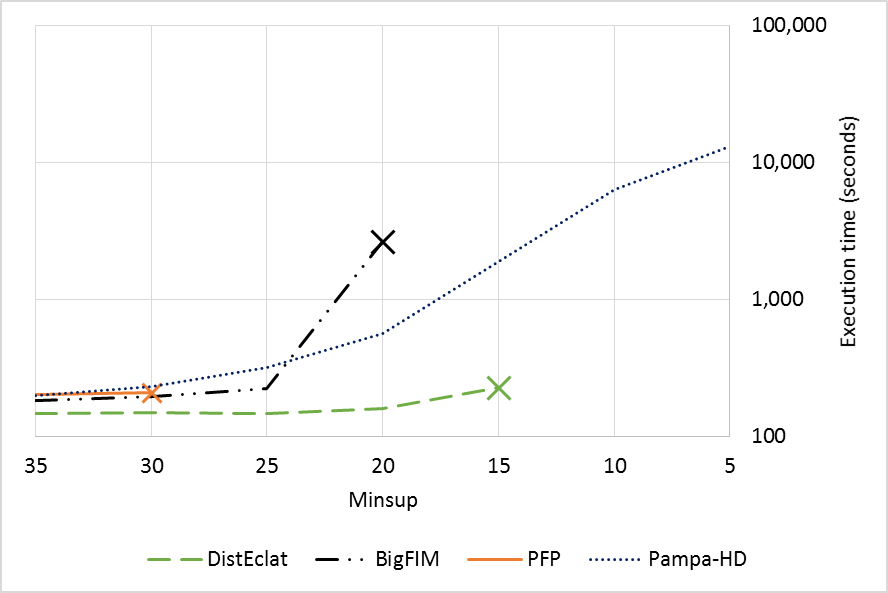
\includegraphics[width=5in]{chapters/pampa/immagini_extension/pems_confronto.png}
\caption{Execution time for different Minsup values on the PEMS-SF dataset (100-rows).}
\label{pems_confronto}
\end{figure}

\begin{figure}[!t]
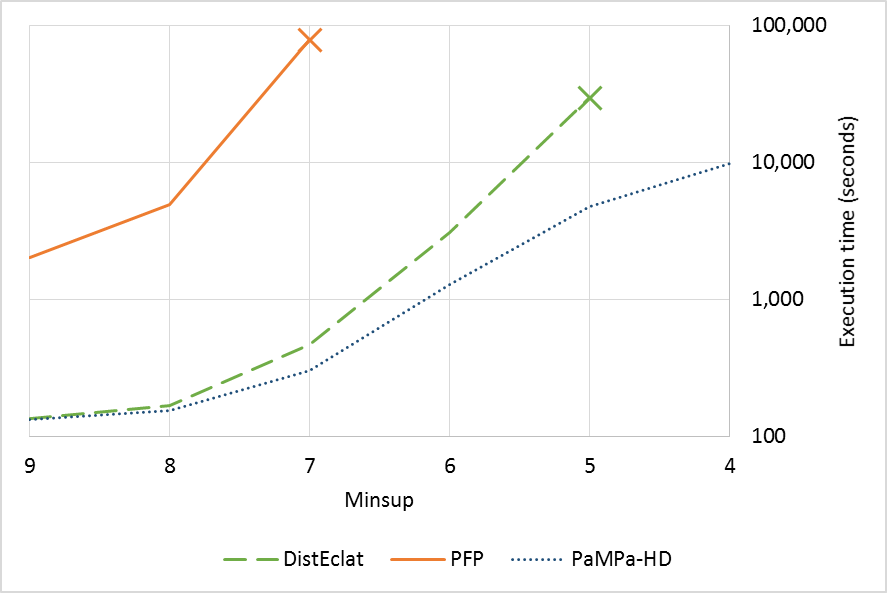
\includegraphics[width=5in]{chapters/pampa/immagini_extension/breast_confronto.png}
\caption{Execution time for different Minsup values on the Breast Cancer dataset.}
\label{breast_confronto}
\end{figure}
The second set of experiments are performed with the Breast
Cancer dataset~\cite{breast_cancer_dataset}.
As reported in Figure~\ref{breast_confronto} (Even in this case, minsup axis is reversed to improve readability, the minsup is absolute), PaMPa-HD is the most reliable and fast approach.
This time, BigFIM is not able to cope even with the highest minsup values, while PFP shows very slow execution times and runs out of memory with a minsup value of 6.
DistEclat is able to achieve good performances but is always slower than PaMPA-HD (with a minsup value equal to 4, it is not able to complete the mining within several days of computation).
From these results, we have seen how traditional best-in-class approaches such as BigFIM, DistEclat and PFP are not suitable for high-dimensional datasets. They are slow and/or not reliable when coping with the curse of dimensionality. PaMPa-HD, instead, demonstrated to be most suitable approach with datasets characterized by a high number of items and a small number of rows.
After the comparison with the state of the art distributed frequent itemset mining algorithms, the next subsections will experimentally analyze the behavior of PaMPa-HD with respect to the number of transactions, number of independent tasks, communication costs and load balancing.
%Because of the algorithm design of our approach, we already know that it is very sensitive with respect to the transactions of the input dataset. It will be interesting to evaluate the impact of the number of independent tasks. This issue is not trivial because adding a task to the computation would not only delivers more resources such as memory or CPU. An additional task leads to split the chunk of the enumeration tree that is explored

%\begin{figure}[!t]
%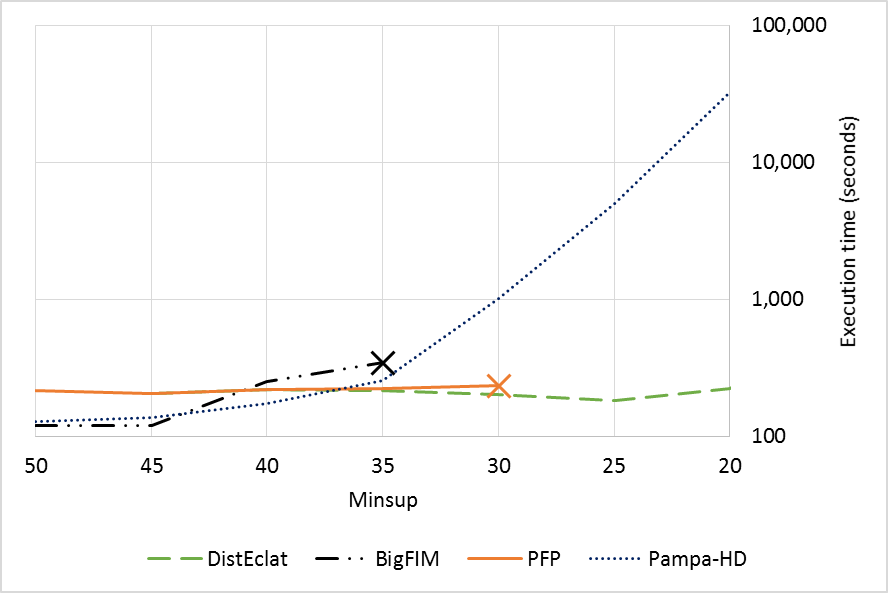
\includegraphics[width=5in]{chapters/pampa/immagini_extension/pems_confronto_200.png}
%\caption{Execution time for different Minsup values on the PEMS-SF dataset (200-rows).}
%\label{pems_confronto_200}
%\end{figure}

\subsection{Impact of the number of transactions}\label{number_rows}
This set of experiments measures the impact of the number of transactions on PaMPa-HD performances. To this aim, the PEMS-SF datasets will be used in three versions (100-rows, 200-rows and full).
The algorithm is very sensitive to this factor: the reasons are related to its inner structure. In fact, the enumeration tree, for construction, is strongly affected by the number of rows. A higher number of rows leads to:
\begin{enumerate}
\item A higher number of branches. As shown in the example in Figure~\ref{running_1}, from the root of the tree, it is generated a new branch for each tid (transaction-id) of the dataset.
\item Longer and wider branches. Since each branch explores its research subspace in a depth-first order, exploring any combination of tids, each branch would result with a greater number of sub-levels (longer) and a greater number of sub-branches (wider)
\end{enumerate}

Therefore, the mining processes related to the 100-rows version and to the 200-rows or the full version of PEMS-SF dataset are strongly different. With a number of rows incremented by, respectively, 200\% and more than 400\%, the mining of the augmented versions of PEMS-SF dataset is very challenging for the enumeration-tree based PaMPa-HD.
%The results in Figure~\ref{pems_confronto_200} and in Figuretoadd confirm these difficulties. With the same range of relative minsup values, BigFIM and PFP show a similar performance with the ones with the reduced version of the dataset (Figure~\ref{pems_confronto}). Their capacity to complete the mining is slightly and gradually reduced by some minsup values points.
%DistEclat, the algorithm which showed the most interesting performances among the ones not designed to fit high-dimensional use cases, shows a very stable behavior for all the mining tasks of the experiments in Figure~\ref{pems_confronto_200}. In the experiments with the full version of the dataset, interestingly, is not able to complete the mine even with a minsup of 50\%.
%PaMPa-HD shows a very strong performance degradation already in the experiments with 200-rows dataset, due to the higher number of transaction. Given $n$ the number of rows of the dataset, the size of the enumeration tree is proportional to $n^2$ \textbf{(che ne pensate?)} (while the approaches used by DistEclat, BigFIM and PFP are sensitive to the number of different items).
The performance degradation is resumed in Figure~\ref{pampa_pems_confronto}, where, for instance, with a minsup of 35\%, the execution times related to the 100-rows and the full version of the PEMS-SF dataset differ of almost two orders of magnitude.

The behavior and the difficulties of PaMPa-HD with datasets with an incremental number of rows, is, unfortunately, predictable. This algorithmic problem represents a challenging and interesting open issues for further developments.
\begin{figure}[!t]
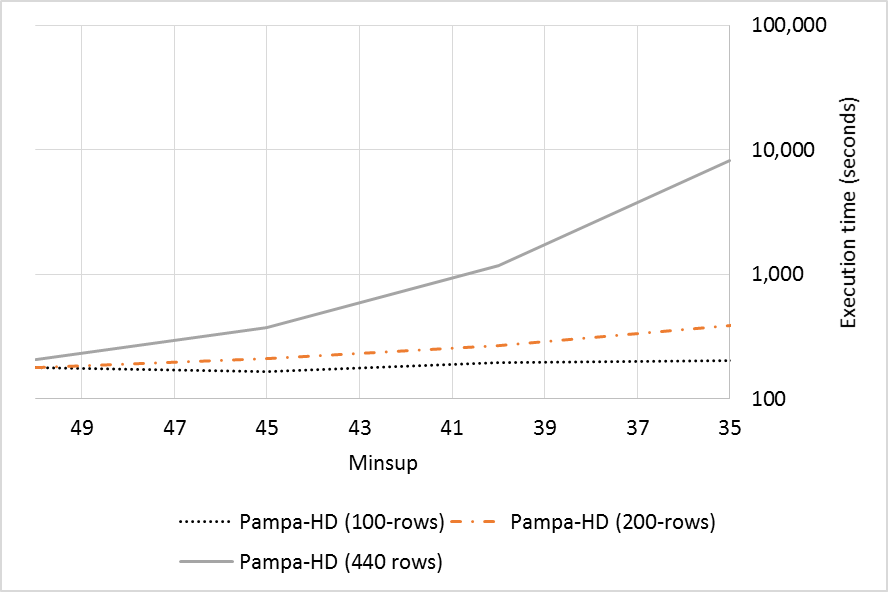
\includegraphics[width=5in]{chapters/pampa/immagini_extension/pampa_pems_confronto.png}
\caption{Execution times for different versions of PEMS-SF for PaMPa-HD.}
\label{pampa_pems_confronto}
\end{figure}





\subsection{Impact of the number of nodes}\label{scalability}
The impact of the number of independent tasks involved in the algorithm execution is a non-trivial issue. 
Adding a task to the computation would not only deliver more resources such as memory or CPU, 
but it also leads to split the chunk of the enumeration tree that is explored by each task. 
On the one hand, this means to reduce the search space to explore, lightening the task load. 
On the other hand, this reduces the state centralized memory and the impact of the related pruning. 
It can be interpreted as a trade-off between the benefits of the parallelism against the state.
In Figure~\ref{scalability_img_pems} and Figure~\ref{scalability_img_breast}, it is reported the behavior of PaMPa-HD with a mining process on the datasets PEMS-SF and Breast Cancer. The minsup values, respectively of 20 and 6, have been chosen in order to highlight the performance differences among the different degree of parallelism and datasets.
Interestingly, the mining on PEMS-SF dataset is less sensitive to the number of reducers, with an execution time that is just halved when the independent tasks included in the computation pass from 1 to 17. The experiment of Breast Cancer instead, Figure~\ref{scalability_img_breast}, shows a stronger performance gain.
As before, the behavior is related to the dataset data distribution which causes the PEMS-SF mining process generating more intermediate tables.
In this case, the advantages related to additional independent nodes into the mining 
is mitigated by the loss of state in the local pruning phase inside the nodes. 
With additional nodes, each node is pushed to a smaller exploration of the search space, 
decreasing the effectiveness of the local pruning.
%PEMS-SF dataset, as discussed in Subsection~\ref{exp_strategies}, mitigates the lack of additional independent nodes with a more aggressive local pruning phase inside the nodes.
These specific results recall a very popular open issue in distributed environments. 
In problems characterized by any kind of ''state'' benefit 
(in this case, the local pruning inside the tasks), 
a higher degree of parallelism does not lead to better performance a priori.
%\textbf{(Riformulare meglio, questo apre questioni interessanti sulla questione di determinare il grado di parallelismo quando si deve lanciare un algoritmo. Finora c'e' stato il forte constraint dei cluster fisici, ora col cloud tutti possono scegliere piu' liberamente. Quindi e' davvero vero che più grande e' il parallelismo migliori saranno le performance? Riprendere il tutto anche nelle conclusioni nelle open issues)}.

\begin{figure}[!t]
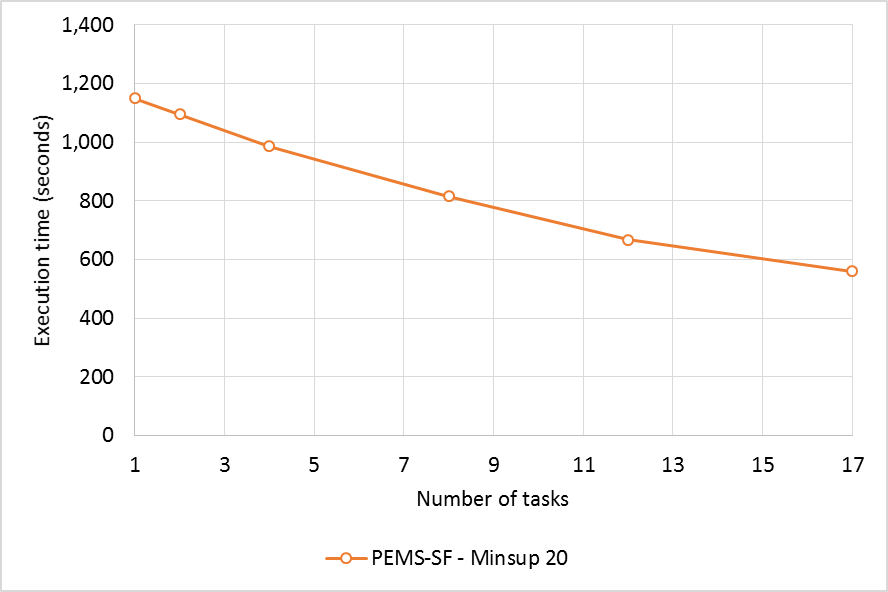
\includegraphics[width=5in]{chapters/pampa/immagini_extension/scalability_pems.png}
\caption{Execution times for PEMS-SF dataset with different number of parallel tasks.}
\label{scalability_img_pems}
\end{figure}

\begin{figure}[!t]
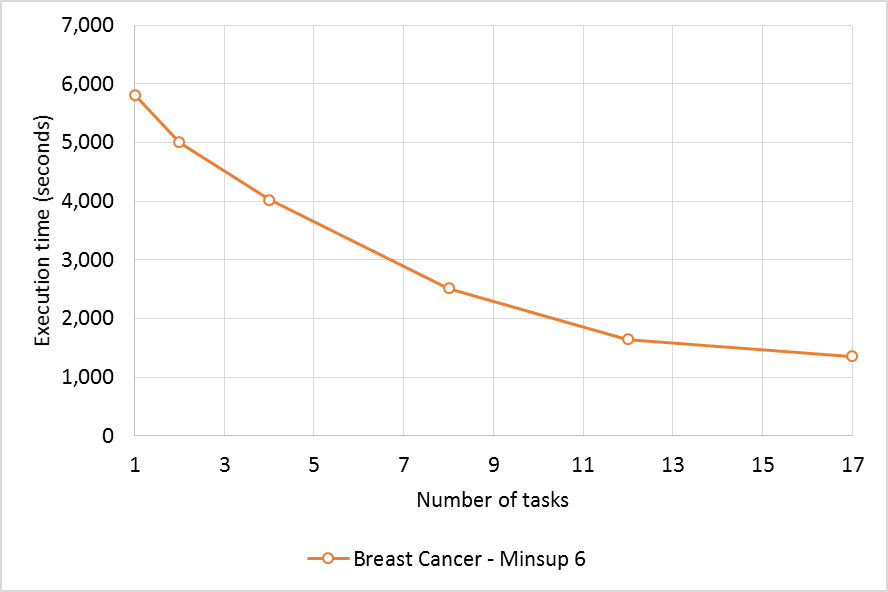
\includegraphics[width=5in]{chapters/pampa/immagini_extension/scalability_breast.png}
\caption{Execution times for Breast Cancer dataset with different number of parallel tasks.}
\label{scalability_img_breast}
\end{figure}


\subsection{Load Balancing and communication costs}\label{communication_cost}
The last analyses are related to the load balancing and the communication costs of the algorithm. These issues represent very important factor in such a distributed environment. Communication costs are among the main bottlenecks for the performance of parallel  algorithms~\cite{Sarma:2013:ULB:2535570.2488334}.
A bad-balanced load among the independent tasks leads to few long tasks that block the whole job.

PaMPa-HD, being based on the Carpenter algorithm, mainly consists on the exploration of an enumeration tree. The basic idea behind the parallelization is to explore the main branches of the tree independently within parallel tasks (Figure~\ref{running_2}). For this reason, each task needs the information (i.e. transposed tables) related to its branch expansion.
The ideal behavior of a distributed algorithm would be to distribute the least amount of data, avoiding redundant informations as much as possible. The reason is that network communications are very costly in a Big Data scenario.
Unfortunately, the structure of the enumeration tree of PaMPa-HD assumes that some pieces of data of the initial dataset is sent to more than one task. For instance, some data related to nodes $TT|_{2}$ and $TT|_{3}$ are the same, because from node $TT|_{2}$ will be generated the node $TT|_{2, 3}$. This is an issue related to the inner structure of the algorithm and a full independence of the initial data for each branch cannot be reached.

In addition, the architecture of the algorithm, with its synchronization phase, increases the I/O costs. In order to prune some useless tables and improve the performance, the mining process is divided in more phases writing the partial results into HDFS.
However, as we have already seen when studying the impact of $max\_exp$ (Figure~\ref{pems_fixed} and Figure~\ref{breast_fixed}), in some cases additional synchronization phases lead to better execution times, despite their related overhead.

In Figure~\ref{comm_cost_pems} and~\ref{comm_cost_breast}, the communication cost during a mining process is reported. The spikes are related to the shuffle phases, in which the redundant tables and closed itemsets are removed.
The flat part of the curve between the spikes is longer in the case of the Breast Cancer dataset because of the adopted strategy. Its mining has been executed with a more aggressive increasing of the $max\_exp$ parameter (steps of 10 for PEMS-SF dataset, 10,000 for Breast Cancer dataset), which leads to a very long period without synchronization phases.


\begin{figure}[!t]
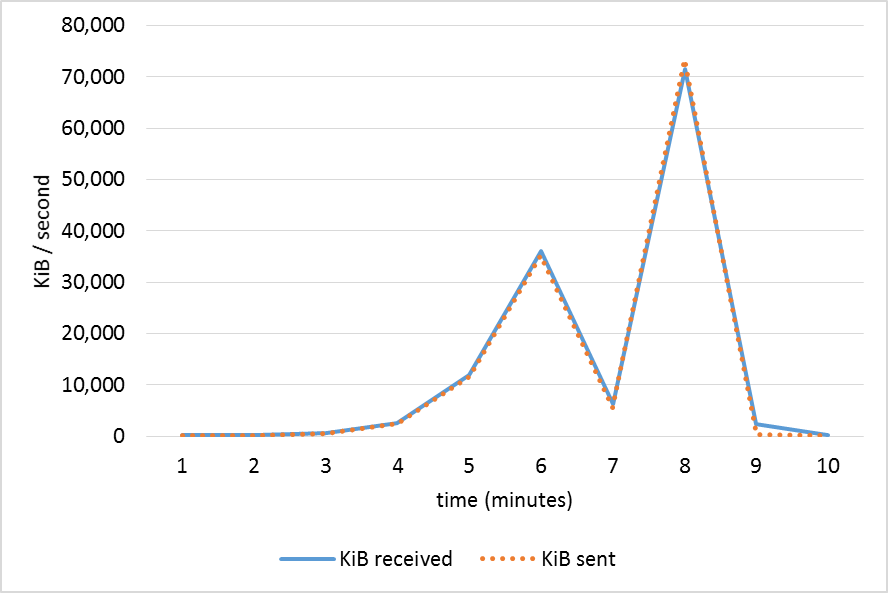
\includegraphics[width=5in]{chapters/pampa/immagini_extension/comm_cost_pems.png}
\caption{Received and sent data in the commodity cluster network during PEMS-SF dataset mining, minsup=20.}
\label{comm_cost_pems}
\end{figure}

\begin{figure}[!t]
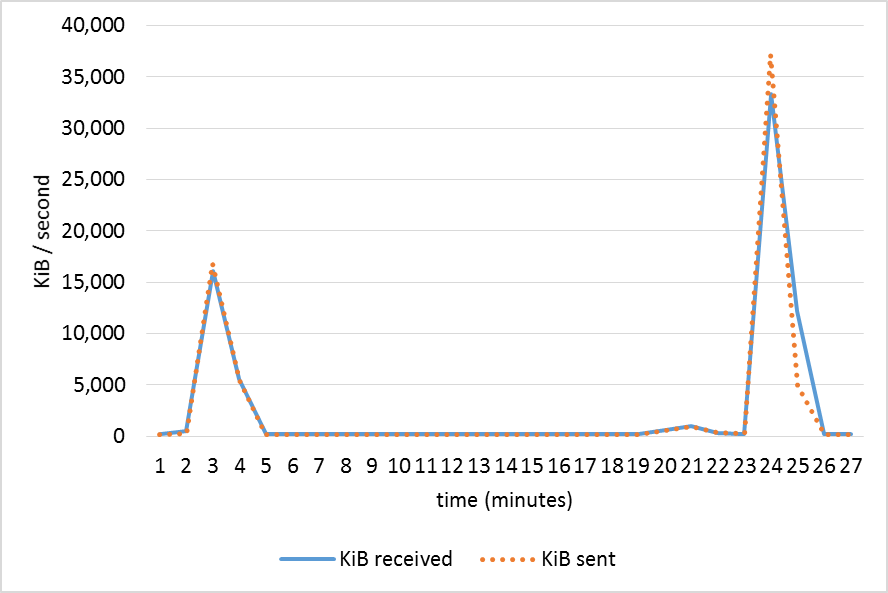
\includegraphics[width=5in]{chapters/pampa/immagini_extension/comm_cost_breast.png}
\caption{Received and sent data in the commodity cluster network during Breast Cancer dataset mining, minsup=6.}
\label{comm_cost_breast}
\end{figure}

The load balancing is evaluated by comparing the execution time of the fastest and slowest tasks related to the iteration job in which this difference is strongest. The most unbalanced phase of the job is, not surprisingly, the mapper phase of the Job 3. This job is iterated until the mining is complete and it is the one more affected by the increase of the $max\_exp$ parameter (iterations characterized by high $max\_exp$ value are likely characterized by long and unbalanced task).
\begin{table}
\begin{center}
\caption{Load Balancing}
\label{load balance final}
\begin{tabular}{ | c | c| c| }
\hline
	Dataset						    & Slowest Task & Fastest Task  \\
							    &  Execution time &  Execution time \\ \hline \hline
	PEMS-SF & 3mins 58 sec & 3mins 37sec \\ \hline
	Breast Cancer & 20mins 33sec & 8mins 42sec\\ \hline
%\multicolumn{2}{|c|}{Task execution time}    & \multicolumn{2}{|c|}{Task execution time}      \\
% & \multicolumn{2}{|c|}{Breast Cancer}    & \multicolumn{2}{|c|}{PEMS-SF}      \\ \hline
%	Maximum expansion threshold &   Min          & Max    &   Min          & Max          \\ \hline
%	100,000,000                 &    7 m                      & 2h 16m 17s &    44s                      & 2h 20m 28s
%  \\ \hline
%10                         &    6m 21s                      &        45m 16s  &   6s                      &        2m 24s
% \\ \hline
\end{tabular}
\end{center}
\end{table}
The difference among the fastest and the slowest mapper is shown in Table~\ref{load balance final}. It is clear that the mining on PEMS-SF dataset is more balanced among the independent tasks. Even in this case, the reason is the different increment value in the Strategy \#1 (10 for PEMS-SF dataset, 10,000 for Breast Cancer dataset). A slower $max\_exp$ increasing leads to more balanced tasks.


%The difference among the fastest and the slowest mapper, as shown by Table~\ref{load balance final}, is not negligible. However, for both the datasets mining, the most unbalanced job is in a phase of the global mining in which there are a lot of input data, which correspond to a number of HDFS chunk greater than the number of mapper. Therefore, even if a long-tailed job does happen, the commodity cluster resources are not completely wasted because new mappers are scheduled as soon as the first ones are processed. This mitigates the load unbalance and the resource lose.




%This section addresses the scalability of PaMPa-HD with respect to the
%number of reducers, since the most heavy operations (i.e.,
%the execution of the ``local'' Carpenter) are executed by the reducers.
%The number of reducers varies from 1 to 18,
%which is the maximum number of tasks that can be run simultaneously
%in the commodity cluster at our disposal.
%The Breast cancer dataset and a minimum absolute
%support threshold equal to 6 have been used.
%As shown in figure~\ref{scalability},
%the increase of the number of reducers has
%a positive impact on the execution time
%when the number of reducers is less than 10.
%The marginal benefits decrease as more reducers are added to the computation.
%Therefore, with more than 10 reducers, the benefits of the load distribution
%are compensated by the decreased effectiveness of the local pruning (i.e., the
%more the load is distributed, the less effective the local pruning is).
% %As already mentioned, the behavior is strictly connected with the considered
% dataset.

%
%\begin{figure}[!t]
%\includegraphics[width=5in]{grafo_scalability.png}
%\caption{Execution time with different numbers of reducers on Breast Cancer dataset with $minsup$=6.}
%\label{scalability}
%\end{figure}





\section{Related work}
\label{Related work}

 \textbf{Already pruned redundant stuff}
As already discussed, Frequent itemset mining represents a
very popular data mining technique
used for exploratory analysis.
Its popularity is witnessed by the high number of approaches
and implementations.
The most popular techniques to extract frequent itemsets
from a transactional datasets are Apriori~\cite{Agr94}, Fp-growth~\cite{Han00} and, even if less popular, Eclat~\cite{Zaki97newalgorithms}.
%Apriori~\cite{Agr94} is a bottom up approach:
%itemsets are extended one item at a time and their frequency is tested against
%the dataset.
%FP-growth~\cite{Han00}, instead, is based on an FP-tree transposition of the
%transactional dataset
%and a recursive divide-and-conquer approach.
These techniques explore the search space enumerating the items.
For this reason, they work very well for datasets
with a small number of items per row,
but their running time increases exponentially
with higher row lengths~\cite{Agr94, Zaki97newalgorithms}.
This behavior is directly inherited by their respective distributed implementations:
Parallel FP-growth~\cite{pfpgrowth},~\cite{citeulike:13636750}, BigFIM and DistEclat~\cite{bigfim}.


%These are not the only distributed and parallel implementations of Frequent Itemset miners.
%\cite{qiu2014yafim} introduces another Apriori-based frequent
%itemset miner. The contribution of this work is focused on the candidates
%handling, which are cached in memory between each iteration.
%In~\cite{zhang2015distributed}, a similar breadth-first approach is introduced, but with the exploitation of a matrix-based pruning in order to significantly reduce the amount of candidates. In~\cite{liang2015sequence}, the breadth-first exploration manner is combined
%with the suffix-based candidate generation.\\
%Finally, for the environments requiring very fast response, some sampling-based techniques have been presented~\cite{riondato2015mining},~\cite{gole2015frequent} and~\cite{Wu2015}. These works are characterized by getting a trade-off between execution time and quality of the results. \\
%While the previous works have been designed for use cases characterized by
%datasets with a large amount of transactions,
As largely discussed, Carpenter algorithm~\cite{Zaki_Carpenter}, 
has been specifically designed to extract frequent itemsets
from high-dimensional datasets (in the order of tens of thousands or more attributes). A detailed introduction to the algorithm is presented in section \ref{Carpenter
algorithm}.
The idea of designing a parallel MapReduce algorithm to efficiently support
itemset mining on high dimensional data was first introduced in~\cite{pampa_v1}.
The PaMPa-HD algorithm significantly enhances the algorithm performance proposed in~\cite{pampa_v1}
by providing (i) a more efficent approach to address synchronization phase, reducing the number of MapReduce jobs; (ii) a
more efficient visit of the transposed tables; (iii) and a set of self-tuning strategies to speed up the performances through a dynamic modification of the $max\_exp$ parameter . Furthermore, this work introduces a wider set of experiment to evaluate, on real datasets, the impact of the number of transaction on the performance, but also communication costs and load balancing, very important in a distributed environment.

Specifically, the original algorithm
exploits an additional independent
synchronization job at each iteration. As already described in
Section~\ref{MapReduce Carpenter}, this implementation includes the
synchronization phase in the Mining Job 3. Therefore, the number of MapReduce
jobs (with their related overhead) are strongly reduced.
Additionally, in order to better exploit the pruning rule in the local Carpenter
iteration in each independent task, all the transposed tables are now processed
(not only expanded) in depth-first order. This strategy decreases the
possibility to explore an useless branch of the tree, i.e. a branch whose
results would be completely overwritten by the closed itemsets obtained by
branches older in depth-first fashion. For instance, the performance improvement from the previous version, measured with Breast Cancer Dataset (minsup=6) is from 6\% to 30\% (depending on the number of independent tasks).
%
%In recent years, the availability of Big Data technologies
%allowed the implementation of these techniques in distributed environments
%such as Apache Hadoop~\cite{HDFS},
%based on the MapReduce paradigm~\cite{ArticoloMapReduceGoogle},
%and Apache Spark~\cite{Zaharia_spark}.
%Parallel FP-growth~\cite{pfpgrowth} is the most popular
%distributed closed frequent itemset mining algorithm.
%The main idea is to process more sub-FP-trees in parallel.
%A dataset conversion is required to make all the FP-trees independent.
%A Spark implementation of Parallel FP-growth has been delivered with MLlib
%Library~\cite{citeulike:13636750}. This version extracts all the frequent
%itemsets and not just the closed ones.
%BigFIM and DistEclat~\cite{bigfim} are two recent methods to extract frequent
%itemsets.
%DistEclat represents a distributed implementation of the Eclat
%algorithm~\cite{Zaki97newalgorithms}
%an approach based on equivalence classes (groups of itemsets sharing the same
%prefixes),
%smartly merged to obtain all the candidates.
%BigFIM is a hybrid approach exploiting both the Apriori and Eclat paradigms.
%BigFIM and DistEclat are divided in two phases. In the first one, the approaches
%use respectively an Apriori-like and Eclat-like strategy to mine the itemsets up
%to a fixed k-length. After that, the itemsets are distributed and used as
%prefixes for the longer itemsets. In the last phase, both
%approaches use Eclat to extract all the closed itemsets.
%In addition,~\cite{qiu2014yafim} introduces another Apriori-based frequent
%itemset miner. The contribution of this work is focused on the candidates
%handling, which are cached in memory between each iteration.
%In~\cite{zhang2015distributed}, a similar breadth-first approach is introduced, but with the exploitation of a matrix-based pruning in order to significantly reduce the amount of candidates. In~\cite{liang2015sequence}, the breadth-first exploration manner is combined
%with the suffix-based candidate generation.
%Finally, for the environments requiring very fast response, some sampling-based techniques have been presented~\cite{riondato2015mining},~\cite{gole2015frequent} and~\cite{Wu2015}. These works are characterized by getting a trade-off between execution time and quality of the results. 
%While the previous works have been designed for use cases characterized by
%datasets with a large amount of transactions,
%Carpenter algorithm~\cite{Zaki_Carpenter}, which inspired PaMPa-HD,
%has been specifically designed to extract frequent itemsets
%from high-dimensional datasets, i.e., characterized by a very large number of
%attributes (in the order of tens of thousands or more).
%The basic idea is to investigate the row set space instead of the itemset
%space.
%%A detailed introduction to the algorithm is presented in section \ref{Carpenter
%%algorithm}.
%The idea of designing a parallel MapReduce algorithm to efficiently support
%itemset mining on high dimensional data was first introduced in~\cite{pampa_v1}.
%The PaMPa-HD algorithm significantly enhances the algorithm performance proposed in~\cite{pampa_v1}
%by providing (i) a more efficent approach to address synchronization phase, reducing the number of MapReduce jobs; (ii) a
%more efficient visit of the transposed tables; (iii) and a set of self-tuning strategies to speed up the performances through a dynamic modification of the $max\_exp$ parameter . Furthermore, this work introduces a wider set of experiment to evaluate, on real datasets, the impact of the number of transaction on the performance, but also communication costs and load balancing, very important in a distributed environment.
%
%This work extends our previous work~\cite{pampa_v1}. The original algorithm
%exploits an additional independent
%synchronization job at each iteration. As already described in
%Section\ref{MapReduce Carpenter}, this implementation includes the
%synchronization phase in the Mining Job 3. Therefore, the number of MapReduce
%jobs (with their related overhead) are strongly reduced.
%Additionally, in order to better exploit the pruning rule in the local Carpenter
%iteration in each independent task, all the transposed tables are now processed
%(not only expanded) in depth-first order. This strategy decreases the
%possibility to explore an useless branch of the tree, i.e. a branch whose
%results would be completely overwritten by the closed itemsets obtained by
%branches older in depth-first fashion. For instance, the performance improvement from the previous version, measured with Breast Cancer Dataset (minsup=6) is from 6\% to 30\% (depending on the number of independent tasks).
%% mi sono riferito all'esperimento di scalabilità del precedente paper.






\section{Applications}
\label{Applications}
%\textbf{Questo tutto vecchio, rifrasare? Lo eliminiamo? Michiardi: solo se
%abbiamo problemi di spazio} Since PaMPa-HD is able to process extremely
%high-dimensional datasets we believe it is suitable for
%many application (scientific) domains.
Since PaMPa-HD is able to process extremely
high-dimensional datasets, it enriches the set of algorithm
able to deal with datasets characterized by a very large variety of features (e.g.~\cite{Vimieiro20141},~\cite{Bermejo201235}).
Consequentely, many fields of applications which exploits frequent itemset to discover hidden correlations and association rules~\cite{KamsuFoguem20131034}
 could benefit of it.
The first example is bioinformatics~\cite{Nahar20131086} and health environments:
researchers in this domain often cope with data structures
defined by a large number of attributes,
which matches gene expressions,
and a relatively small number of transactions,
which typically represent medical patients or tissue samples.
Furthermore, smart cities and computer vision applications
are two important domains which can benefit
from our distributed algorithm,
thanks to their heterogeneous nature.
Another field of application is the networking domain.
%This environment is surely the one with the major amount and types of
%collected data.
%The reason is related to the high number of available information sources
%and the easiness to collect information.
Some examples of interesting high-dimensional dataset are
URL reputation, advertisements, social networks and search engines.
One of the most interesting applications,
which we plan to investigate in the future,
is related to internet traffic measurements.
Currently, the market offers an interesting variety of internet packet sniffers
like~\cite{Tstat},~\cite{netflow}. Collected datasets, that include traffic flows in which the item are flow
attributes (\cite{trustcom2013},~\cite{fontas_AR},~\cite{Netmine}), represent an appealing domain where
PaMPa-HD can be efficiently exploited.
are already a very promising application domain
for data mining techniques.
% %These datasets are characterized by a large number of transactions (usually
% millions per hour) and few tens of attributes.
% %However, we plan to merge all the transactions within a time window and apply
% some data mining techniques,
% %such as our Distributed Carpenter implementation.
% %The target would be to extract some deeply hidden knowledge, if there is,
% related to network status,
% %trying to early detect or predict anomalous events or congestions.



\section{Conclusion} \label{Conclusion}
This Chapter introduced PaMPa-HD,
a novel frequent closed itemset mining algorithm
able to efficiently parallelize the itemset extraction from extremely
high-dimensional datasets.
Experimental results show its good scalability
and its efficient performance in dealing with real-world datasets
characterized by up to 8 millions different items
and, above all, an average number of items per transaction
over hundreds of thousands,
on a small commodity cluster of 5 nodes.
PaMPa-HD outperforms state-of-the-art algorithms, by showing a better
scalability than all popular distributed approaches, such as PFP,
DistEclat and BigFIM.
%Further developments of the framework can be related to the introduction of new
%pruning rules in specific use cases. This pruning,
%so far related to the post processing phase, would avoid the processing of
%useless data.
Further developments of the algorithm can be related to the analysis of the trade-off between the benefits of the scalability and the ones related to the local state. 
In addition, future works could analyze the introduction of better load balancing mechanisms. The increasing $max\_exp$ parameter introduced by the self-tuning strategies leads to a degradation of the load balancing between the parallel tasks of the job. As shown in Table~\ref{load balance breast}, higher $max\_exp$ values decrease load balancing (i.e. only few tasks running), wasting the resources assigned to the tasks that are already complete.
Forcing the synchronization phase after a fixed period of time would limit the amount of time in which the resources are not completely exploited. From the algorithmic point of view, this is not a loss, since the tables are expanded in a depth-first fashion. The last tables, hence, are the ones with highest probability to be pruned. This future development, therefore, would analyze the choice of the \textit{time-out} which forces the synchronization phase.

%\textbf{\#Daniele @Fabio: non c'e' nessun altro futur work che ti viene in mente? solo pruning?
%Pietro diceva nei commenti di riprendere le open issue della scalabilita (vedi esperimento), magari possiamo mettere qualcosa su quello, tipo ridurre l'impatto del local state che limita la scalabilita...? Fabio: ci penso, tanto è per dire. Quello del local state secondo me è abbastanza insormontable e caratterizza tutti gli alg distribuiti. ma ci sta. La mia idea sarebbe di cercare  un modo per non fare la distribuzione per ramo ma per profondità. Lo scrivo io.}
%We plan to apply this approach in the network data analysis domain
%and to develop an Apache Spark implementation.
%We also plan to improve the expansion threshold selection:
%an auto-tuning mechanism based on the specific data distribution
%might further unleash the algorithm potential.


\section*{Acknowledgement}
The research leading to these results has received funding from the European
Union under the FP7 Grant Agreement n. 619633 (Project ``ONTIC'').
\\
%% The Appendices part is started with the command \appendix;
%% appendix sections are then done as normal sections
%% \appendix

%% \section{}
%% \label{}

%% If you have bibdatabase file and want bibtex to generate the
%% bibitems, please use
%%
%%  \bibliographystyle{elsarticle-num} 
%%  \bibliography{<your bibdatabase>}

%% else use the following coding to input the bibitems directly in the
%% TeX file.

\bibliographystyle{elsarticle-num}
\bibliography{biblio}{}

%% \bibitem{label}
%% Text of bibliographic item



\end{document}
%\endinput
%%
%% End of file `elsarticle-template-num.tex'.
